\chapter{Dispersed-phase simulations in liquid JICF}
	\label{ch6:jicf_lgs_simulations}


%Describe here all our results from the lagrangian simulations:
%
%\begin{itemize}
%
%	\item Effects of applying full workflow: w/wo ALM, w/wo secondary atomization ...
%	
%	\item Mesh convergence study: specify it
%	
%	\item Validation with experiments
%	
%	\item Mass conservation issues: lagrangian tracking, etc. 
%	
%
%\end{itemize}


\section{Introduction}

This chapter presents results from lagrangian simulations performed with the SLI models described in Chapter \ref{ch4:sli_development}. The test case used is the academic JICF of \citeColor[becker_breakup_2002], for which resolved simulations of the atomization process were detailed in Chapter \ref{ch5:jicf_resolved_simulations}. Data for these computations are used to build the injectors in order to run dispersed phase simulations in the same configuration, which are shown to be less computationally expensive than the resolved ones. \hl{...}


\section{Computational setup}

The geometry replicating the experimental test bench is the same than the one used for the resolved simulations, depicted in Figure \ref{fig:numerical_setup_maquette_JICF_DLR}. The operating points simulated are the ones from Table \ref{tab:jicf_operating_conditions}. Regarding the mesh employed, it was shown in $\S$\ref{sec:ch5_initial_conditions} that an element size of $\Delta x = 0.5$ mm allows to transport the estimated turbulence in these cases. Nevertheless, the simulations from Chapter \ref{ch5:jicf_resolved_simulations} use a mesh with this cell size only inside the plenum upstream and around the injector, while downstream the injector the mesh size is enlarged as there is no liquid at this region. This mesh was shown in Figure \ref{fig:jicf_dlr_mesh}. In the lagrangian simulations performed in this chapter, injection is performed at the sampling planes downstream the injector seen in Figure \ref{fig:jicf_IBs_sketch_discretization}, and the region of interest extends up to a location at $x = 80$ mm downstream the injector, which corresponds to the location where the experiments from \citeColor[becker_breakup_2002] report results on fluxes and SMD. Therefore, lagrangian simulations use a baseline cell size of $\Delta x = 0.5$ mm in the plenum from the gaseous inlet up to $x = 85$ mm downstream the injector in order to allow for turbulent transport up to the experimental validation plane (located at $x = 80$ mm). The mesh used, shown in Figure \ref{fig:jicf_dlr_mesh_LGS}, is composed of $74 \cdot 10^6$ elements, being therefore heavier than the baseline mesh employed for the resolved simulations but eventually lighter due to the lack of AMR (see the increase of element size in the resolved simulations at Figure \ref{fig:JICF_nelem_increase_t_0_to_2}, which shows that the smallest mesh obtained for a established jet contains $200 \cdot 10^6$ elements). Liquid particles are injected in this mesh as lagrangian point-particles whose dynamics follow the equations from  $\S$\ref{sec:ch3_EL_formalisms}. The energy equation is not considered since the test bench is at ambient temperature and evaporation does not take place.

\clearpage


%The geometry replicating the experimental test bench is the same than the one used for the resolved simulations, depicted in Figure \ref{fig:numerical_setup_maquette_JICF_DLR}. The operating points simulated are the ones from Table \ref{tab:jicf_operating_conditions}. Regarding the mesh employed, it was shown in $\S$\ref{sec:ch5_initial_conditions} that an element size of $\Delta x = 0.5$ mm allows to transport the estimated turbulence in these cases. Nevertheless, the simulations from Chapter \ref{ch5:jicf_resolved_simulations} use a mesh with this cell size only inside the plenum upstream and around the injector, while downstream the injector the mesh size is enlarged as there is no liquid at this region. This mesh was shown in Figure \ref{fig:jicf_dlr_mesh}. In the lagrangian simulations performed in this chapter, injection is performed at the sampling planes downstream the injector seen in Figure \ref{fig:jicf_IBs_sketch_discretization}, and the region of interest extends up to a location at $x = 80$ mm downstream the injector, which corresponds to the location where the experiments from \citeColor[becker_breakup_2002] report results on fluxes and SMD. Therefore, lagrangian simulations use a baseline cell size of $\Delta x = 0.5$ mm in the plenum from the gaseous inlet up to $x = 85$ mm downstream the injector. Furthermore, the mesh is refined \hl{in the region immediately downstream the injection nozzle to} $\Delta x = 0.3$ mm to allow for a better resolution of the gaseous field perturbed by the ALM, as the turbulent structures from the resolved simulations reported in $\S$\ref{ch5:subsec_turbulent_structures_in_gaseous_field} have smaller characteristic sizes than the turbulence further upstream. It is, however, worth to keep in mind that the gaseous field close to the interface was refined in the resolved simulations to the interface mesh size, allowing for a better resolution of turbulence. This refinement is not available in the dispersed phase simulations, therefore the refinement to $\Delta x = 0.3$ mm. The mesh used, shown in Figure \ref{fig:jicf_dlr_mesh_LGS}, is composed of \textbf{XX} elements, being therefore larger than the baseline mesh employed for the resolved simulations but eventually cheaper due to the lack of AMR, as simulations. Liquid particles are injected in this mesh as lagrangian point-particles whose dynamics follow the equations from  $\S$\ref{sec:ch3_EL_formalisms}. The energy equation is not considered since the test bench is at ambient temperature and evaporation does not take place.

\begin{figure}[h!]
	\centering
	\includeinkscape[inkscapelatex=false,scale=0.8]{./part2_developments/figures_ch6_lagrangian_JICF/jicf_mesh_LGS}
	\caption{Mesh employed for dispersed-phase simulations of the full configuration from Figure \ref{fig:numerical_setup_maquette_JICF_DLR}}
	\label{fig:jicf_dlr_mesh_LGS}
\end{figure}


%\section{Evaporation phenomena}
%
%\textbf{Note: this analysis could perfectly be in the previous chapter}.
%
%As indicated in Table \ref{tab:jicf_operating_conditions}, the temperatures of both liquid kerosene and gaseous air are low (290 and 288 K respectively) and there is not direct evaporation of fuel. Nevertheless, some evaporation can occur at ambient temperature if the vapour pressure of the liquid is lower than the ambient pressure. In the experiments, the ambient pressure is $p_g = 6$ bar, while the vapour pressure of kerosene at $288$ K is $p_{vap} = 0.003$ bar \citepColor[shepherd_flash_2000]. Therefore, evaporation might be possible.
%
%It is tested that ... Two characteristic times are used in the low We case (since the lowest velocity is found there, and the droplets take more time to reach the validation plane at 80 mm)/
%
%\begin{itemize}
%
%	\item The time that a droplet takes to reach the plane x = 80 mm. From the SPS results in $\S$\textbf{??} (or Table \textbf{??}), the first droplets at x = 10 mm are obtained at $t_{resolv} = 0.3$ ms after injection. Then, the first droplets injected at this location in the lagrangian simulations reach the validation plane after $t_\mathrm{lagr} = $ ms. Hence, a characteristic time defined as the :
%	
%	\begin{equation}
%	\tau_{validation} = t_{resolv}  + t_\mathrm{lagr}
%	\end{equation}
%	
%	\item Evaporation time rate is used by means of the $d^2$ law. This law that the square of the droplet's diameter diminishes linearly with time:
%	
%	\begin{equation}
%	\label{eq:d2_law}
%	d^2 \left( \right) = d_0^2 - K t
%	\end{equation}
%	
%	
%	where $K$ is the evaporation rate and $d_0$ the initial diameter of the droplet. The value K ... (see 2006 Ghassemi).
%	
%	
%	\text{NAH}. The evolution in diameter after a given time $t$ can then be obtained as:
%	
%	\begin{equation}
%	\Delta d^2 = d_0^2 - d^2 \left( \right) = K t
%	\end{equation}
%	
%
%\end{itemize}

\section{Experimental results from literature}
\label{sec:ch6_experimental_results}

The study from \citeColor[becker_breakup_2002] reports results on the droplets average size SMD and the liquid volume fluxes in the plane $x = 80$  mm perpendicular to the crossflow. In the resolved simulations of Chapter \ref{ch5:jicf_resolved_simulations} the liquid spray could not reach this location: the increase in mesh size due to a continuous liquid injection and formation of droplets due to atomizatio yielded computations unfeasible if liquid was allowed to travel too far downstream, and hence the liquid domain was restricted up to $x = 10, 15$ mm for the fine and coarse resolutions respectively. This limitation does not apply in the dispersed phase simulations, which can be transported up to the outlet of the domain due to their lower cost compared to the resolved ones. Therefore, the dispersed phase simulations will be compared to the experimental results presented at 80 mm.

Experiments results from PDA measurements can be found in the articles \citeColor[becker_breakup_2002] and \citeColor[rachner_modelling_2002]. Among those, quantitative maps of SMD and volume flux are given, which are shown in Figure \ref{fig:maps_Becker_expe_results}. For both operating points, the volume flux shows a circumferential pattern where the largest flux is located at the center and is reduced radially. Most of the fuel is then located at the center of the spray plume, which is a common feature in liquid jets in crossflow \citepColor[wu_spray_1998]. The maximum value of volume flux is lower for the low Weber case than in the high Weber one, which is expected since the injected liquid mass flow rate is lower for the former than for the later to keep the same momentum flux ratio $q$ in both cases, as Table \ref{tab:jicf_operating_conditions} shows. Regarding the $SMD$, both maps show a ballistic, layered profile where the largest droplets are located in the top part of the spray. This is due to the higher inertia of the biggest droplets produced, which penetrate further than the smallest ones \citepColor[wu_breakup_1997]. In general, $SMD$ values are larger in the low Weber case since the dynamic pressure (or equivalently, the gaseous velocity) is lower, and the size of the droplets produced were found to be highly dependent on this parameter \citepColor[becker_breakup_2002].


%\begin{figure}[h!]
%\flushleft
%\begin{subfigure}[b]{0.4\textwidth}
%	\centering
%   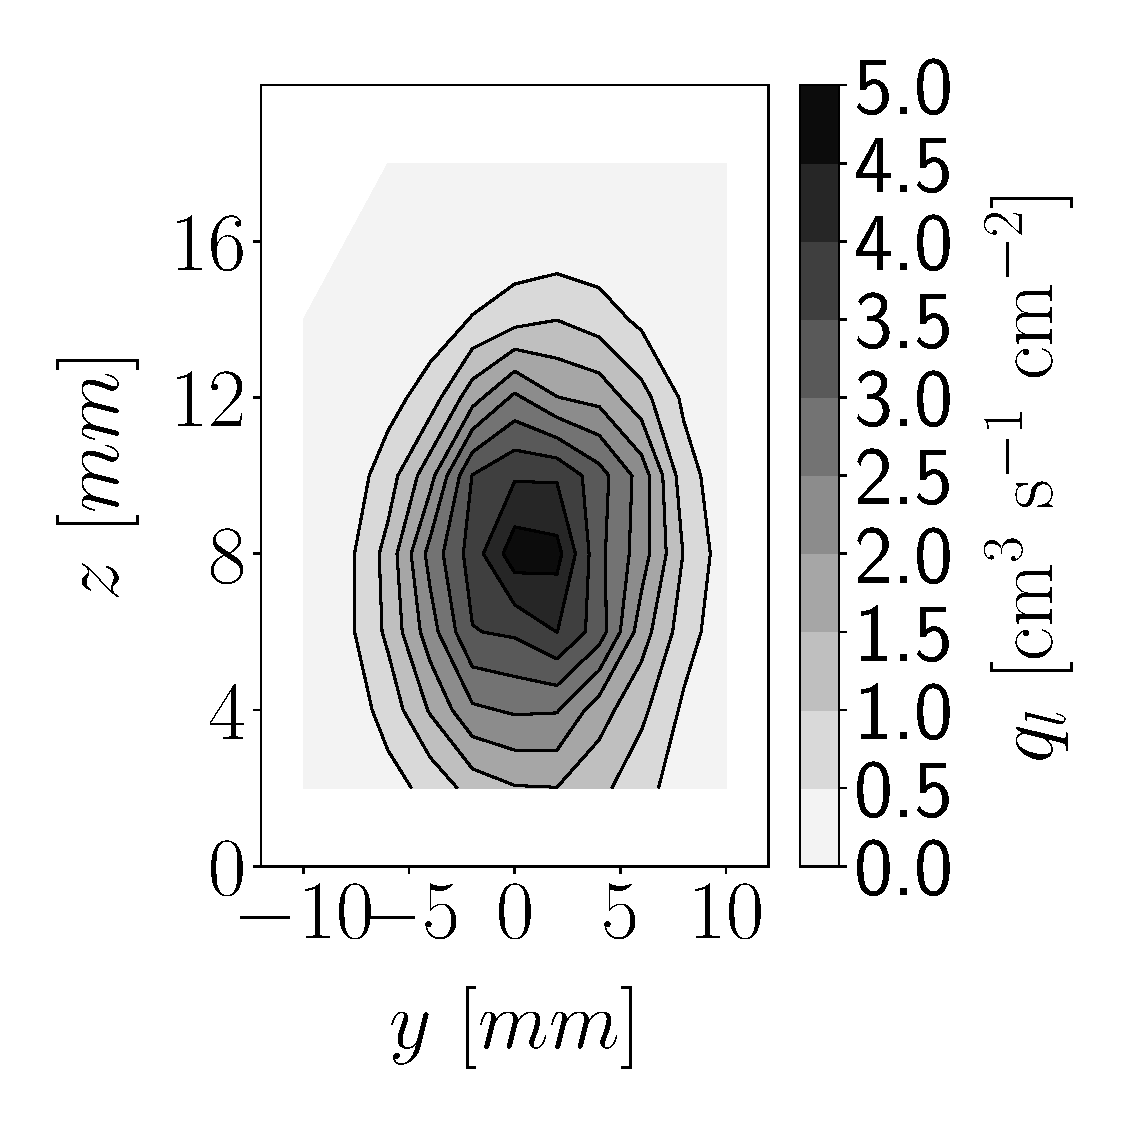
\includegraphics[scale=0.2]{./part2_developments/figures_ch6_lagrangian_JICF/expe_results/map_flux_UG100}
%   \hspace{-0.1in}
%   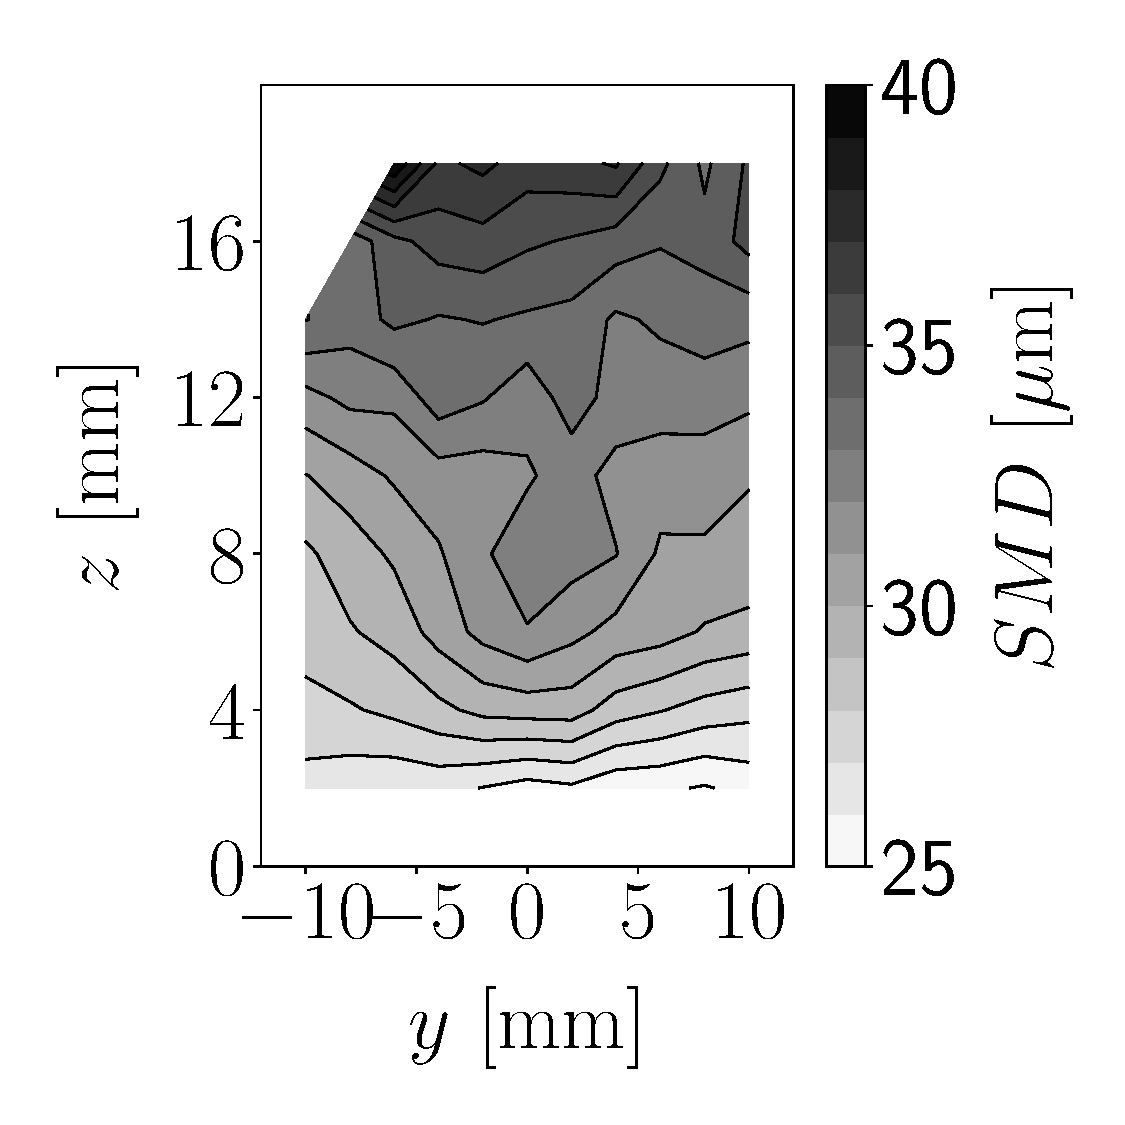
\includegraphics[scale=0.2]{./part2_developments/figures_ch6_lagrangian_JICF/expe_results/map_SMD_UG100}
%   \caption{Low Weber number operating point.}
%   %\label{} 
%\end{subfigure}
%\begin{subfigure}[b]{0.4\textwidth}
%	\flushleft
%   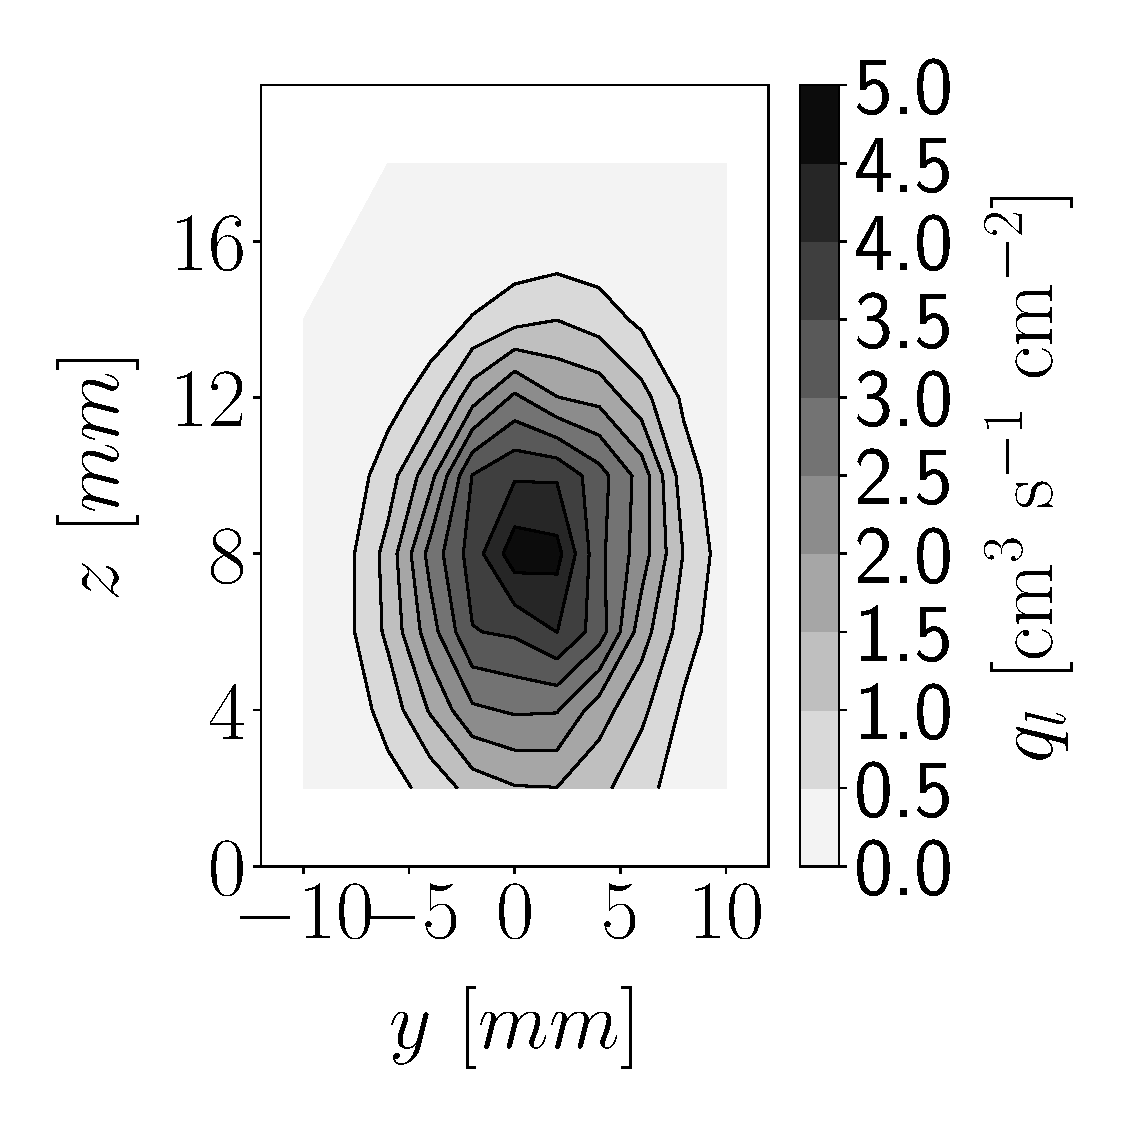
\includegraphics[scale=0.1]{./part2_developments/figures_ch6_lagrangian_JICF/expe_results/map_flux_UG100}
%   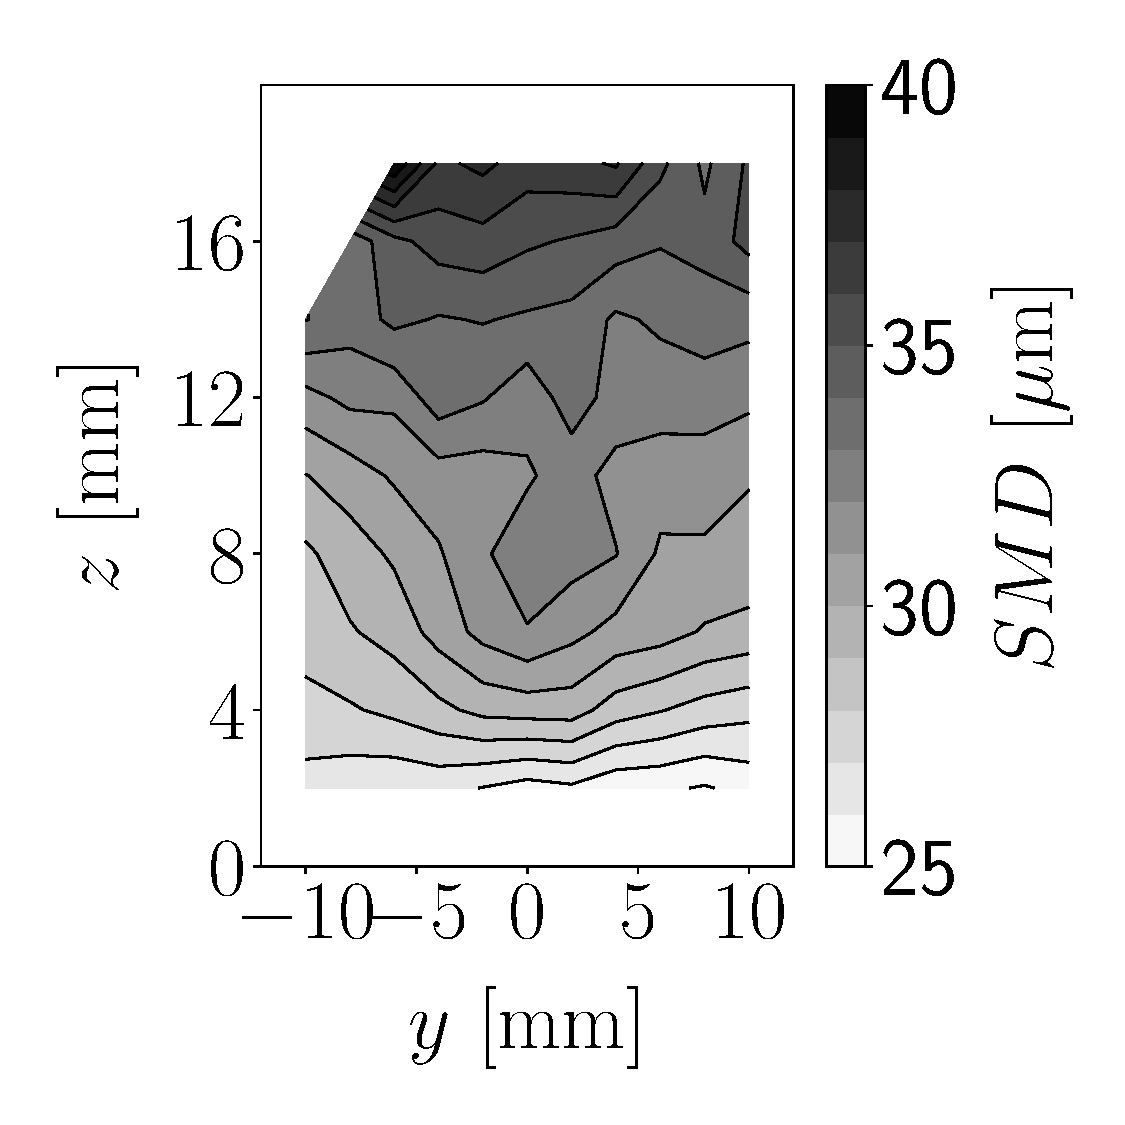
\includegraphics[scale=0.1]{./part2_developments/figures_ch6_lagrangian_JICF/expe_results/map_SMD_UG100}
%   \caption{High Weber number operating point.}
%   %\label{} 
%\end{subfigure}
%\caption{SMD and volume flux maps obtained experimentally by \citeColor[becker_breakup_2002] at a location $x = 80$ mm downstream the liquid injector.}
%\label{fig:maps_Becker_expe_results}
%\end{figure}


\begin{figure}[h!]
\flushleft
\begin{subfigure}[b]{0.45\textwidth}
	\flushleft
   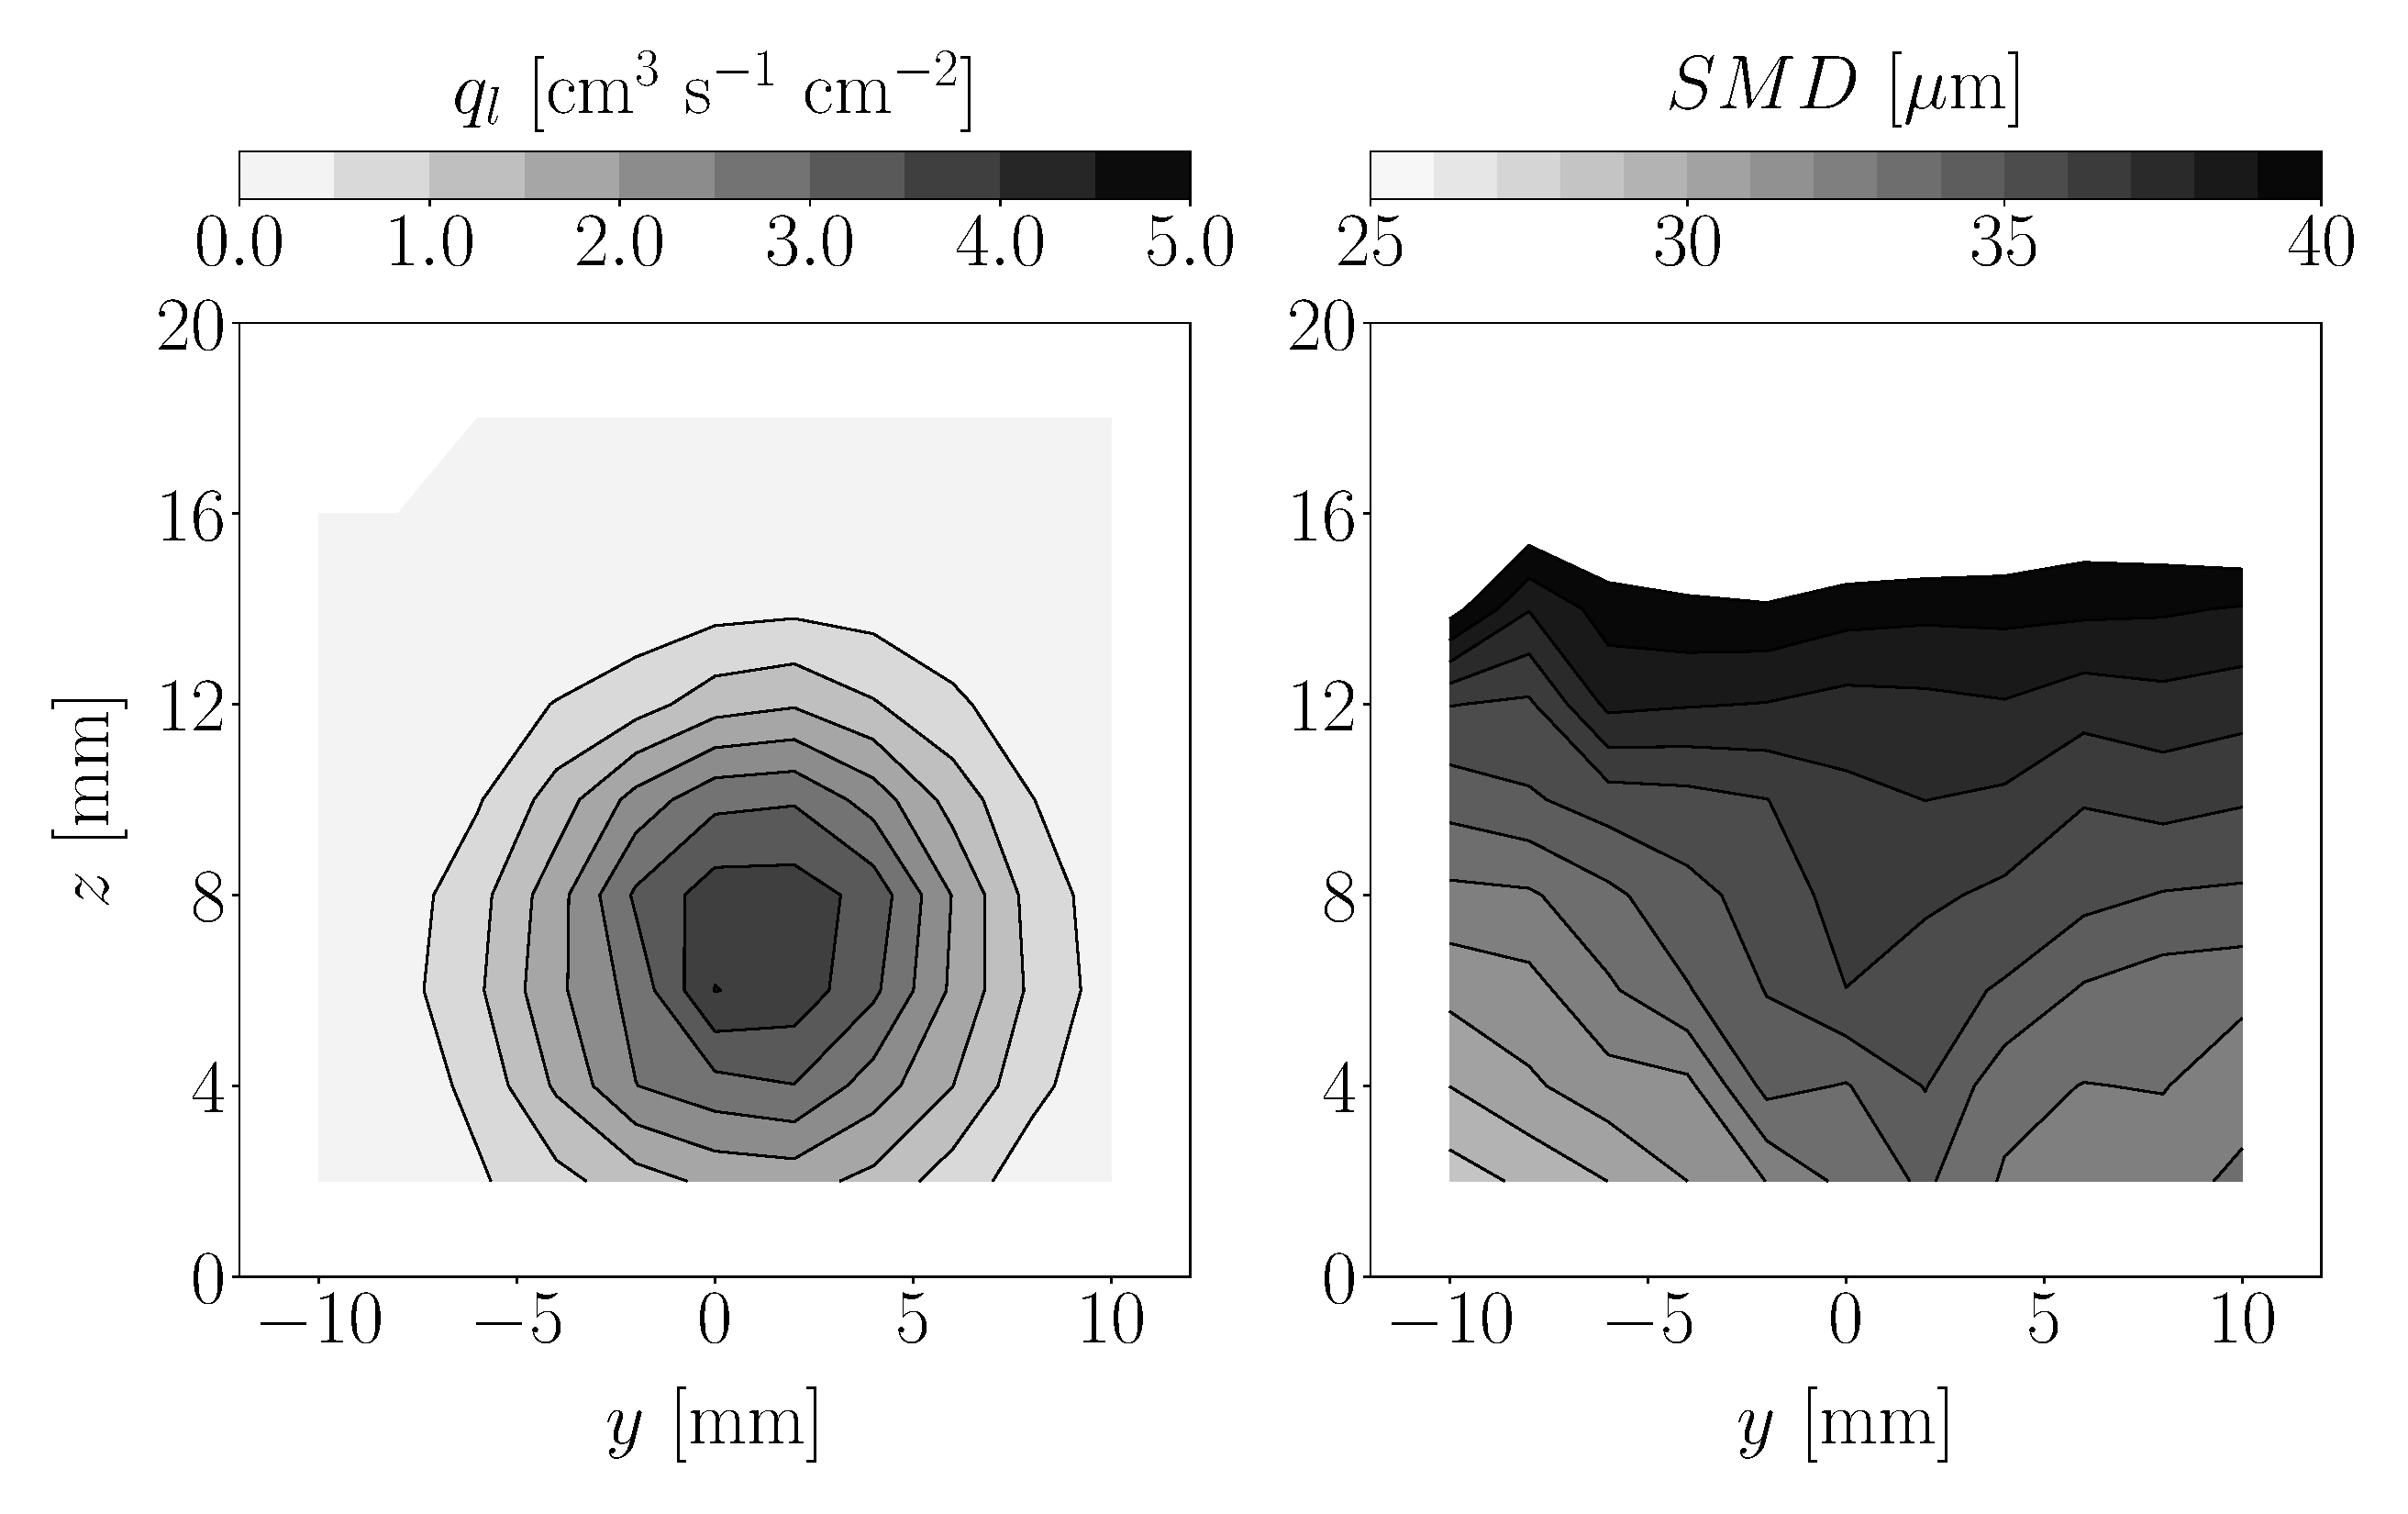
\includegraphics[scale=0.185]{./part2_developments/figures_ch6_lagrangian_JICF/expe_results/maps_UG75}
   \caption{Low Weber number operating point.}
   %\label{} 
\end{subfigure}
\hspace{0.3in}
\begin{subfigure}[b]{0.45\textwidth}
	\centering
   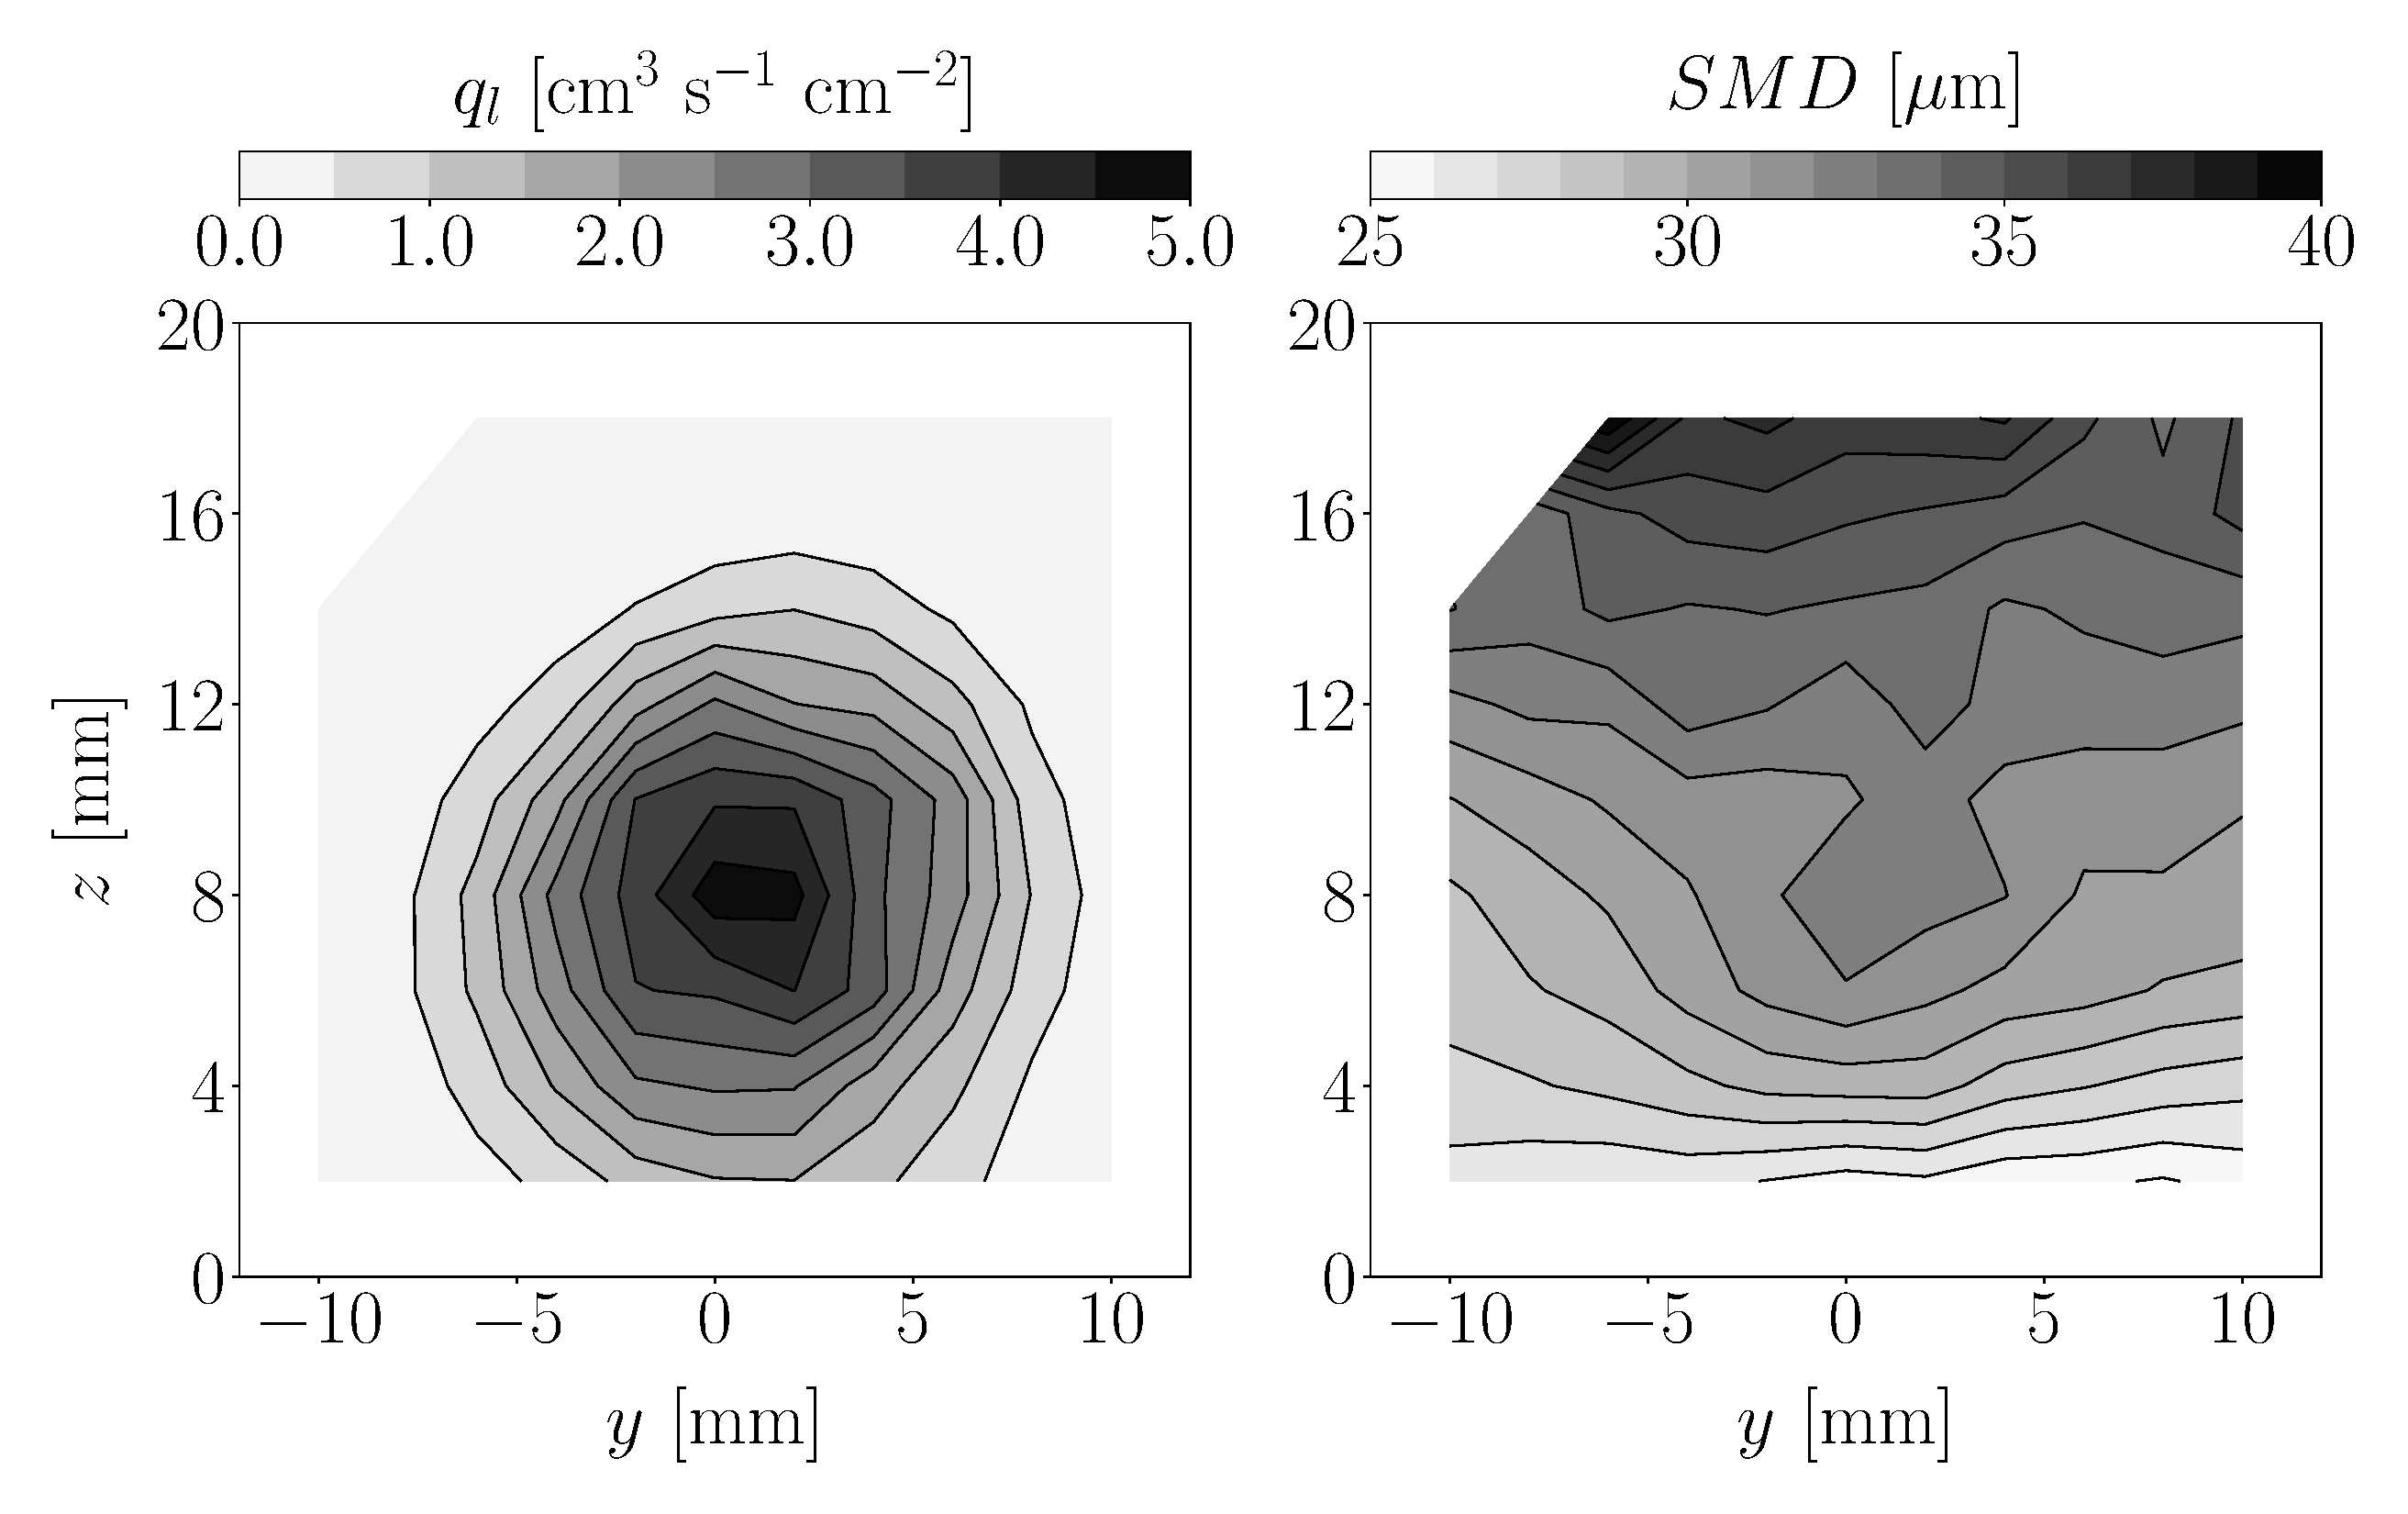
\includegraphics[scale=0.19]{./part2_developments/figures_ch6_lagrangian_JICF/expe_results/maps_UG100}
   \caption{High Weber number operating point.}
   %\label{} 
\end{subfigure}
\caption{SMD and volume flux maps obtained experimentally by \citeColor[becker_breakup_2002] at a location $x = 80$ mm downstream the liquid injector.}
\label{fig:maps_Becker_expe_results}
\end{figure}

Complementary to the maps, qualitative results are also present in the literature which can also be used for validation. These ones are given as the integrated profiles of the liquid volume flux and flux-averaged $SMD$ over the $z$ and $y$ directions, which are then respectively dependent on $y$ and $z$. The equations to obtain such measures are given by Eqs. (\ref{eq:integrated_results_Becker_expe_results}):


\begin{subequations}
\label{eq:integrated_results_Becker_expe_results}
\begin{align}
\langle q_l \left( z \right) \rangle = \frac{1}{L_y} \int_0^{L_y} q_l \left( y, z \right) dy    & ~~~~  ; & \langle SMD \left( z \right) \rangle = \frac{1}{L_y \langle q_l \left( z \right) \rangle} \int_0^{L_y} q_l \left( y, z \right) SMD \left( y, z \right) dy \\
\langle q_l \left( y \right) \rangle = \frac{1}{L_z} \int_0^{L_z} q_l \left( y, z \right) dz    & ~~~~  ; & \langle SMD \left( y \right) \rangle =  \frac{1}{L_z \langle q_l \left( z \right) \rangle} \int_0^{L_z} q_l \left( y, z \right) SMD \left( y, z \right) dz
\end{align}
\end{subequations}


%\begin{equation}
%\langle q_l \left( z \right) \rangle = \frac{1}{L_y} \int_0^{L_y} q_l \left( y, z \right) dy ~~~~; ~~~~ \langle SMD \left( z \right) \rangle = \frac{1}{L_y \langle q_l \left( z \right) \rangle} \int_0^{L_y} q_l \left( y, z \right) SMD \left( y, z \right) dy
%\end{equation}
%
%\begin{equation}
%\langle q_l \left( y \right) \rangle = \frac{1}{L_z} \int_0^{L_z} q_l \left( y, z \right) dz ~~~~; ~~~~ \langle SMD \left( y \right) \rangle = \frac{1}{L_z \langle q_l \left( z \right) \rangle} \int_0^{L_z} q_l \left( y, z \right) SMD \left( y, z \right) dz
%\end{equation}

The application of these equations to the experimental results yield the curves from Figure \ref{fig:integrated_results_Becker_expe_results}. The integrated volume flux over $y$ (Figure \ref{fig:integrated_results_Becker_expe_results_over_y}) shows an increase of the volume flux from the bottom part of the spray (PDA measurements closer to wall, for $z < 2$ mm, could not be performed \citeColor[becker_breakup_2002]) until the spray center, where the maximum flux is reached. Then, the flux decreases with $z$ until there is no more liquid present. Flux values are generally larger for the high $We$ point than for the low $We$ one, and the quantity of liquid extends up to further upstream for the former than for the latter due to its larger liquid velocity at injection. Regarding the SMD profiles, both cases follow a ballistic behaviour. The spray of the high $We$ point contains droplets of larger mean size than the low $We$ one.

With respect to the profiles integrated over $z$ (Figure \ref{fig:integrated_results_Becker_expe_results_over_z}), both SMD and flux lines follow parabollic profiles with the largest values present at $y = 0$, i.e. the coordinate for which the largest fluxes are found. The behaviour of the profiles depending on the operating point follow the same tendencies than in Figure \ref{fig:integrated_results_Becker_expe_results_over_y}: lower fluxes and larger droplets for the low $We$ case.



\begin{figure}[h!]
\flushleft
\begin{subfigure}[b]{0.45\textwidth}
	\flushleft
   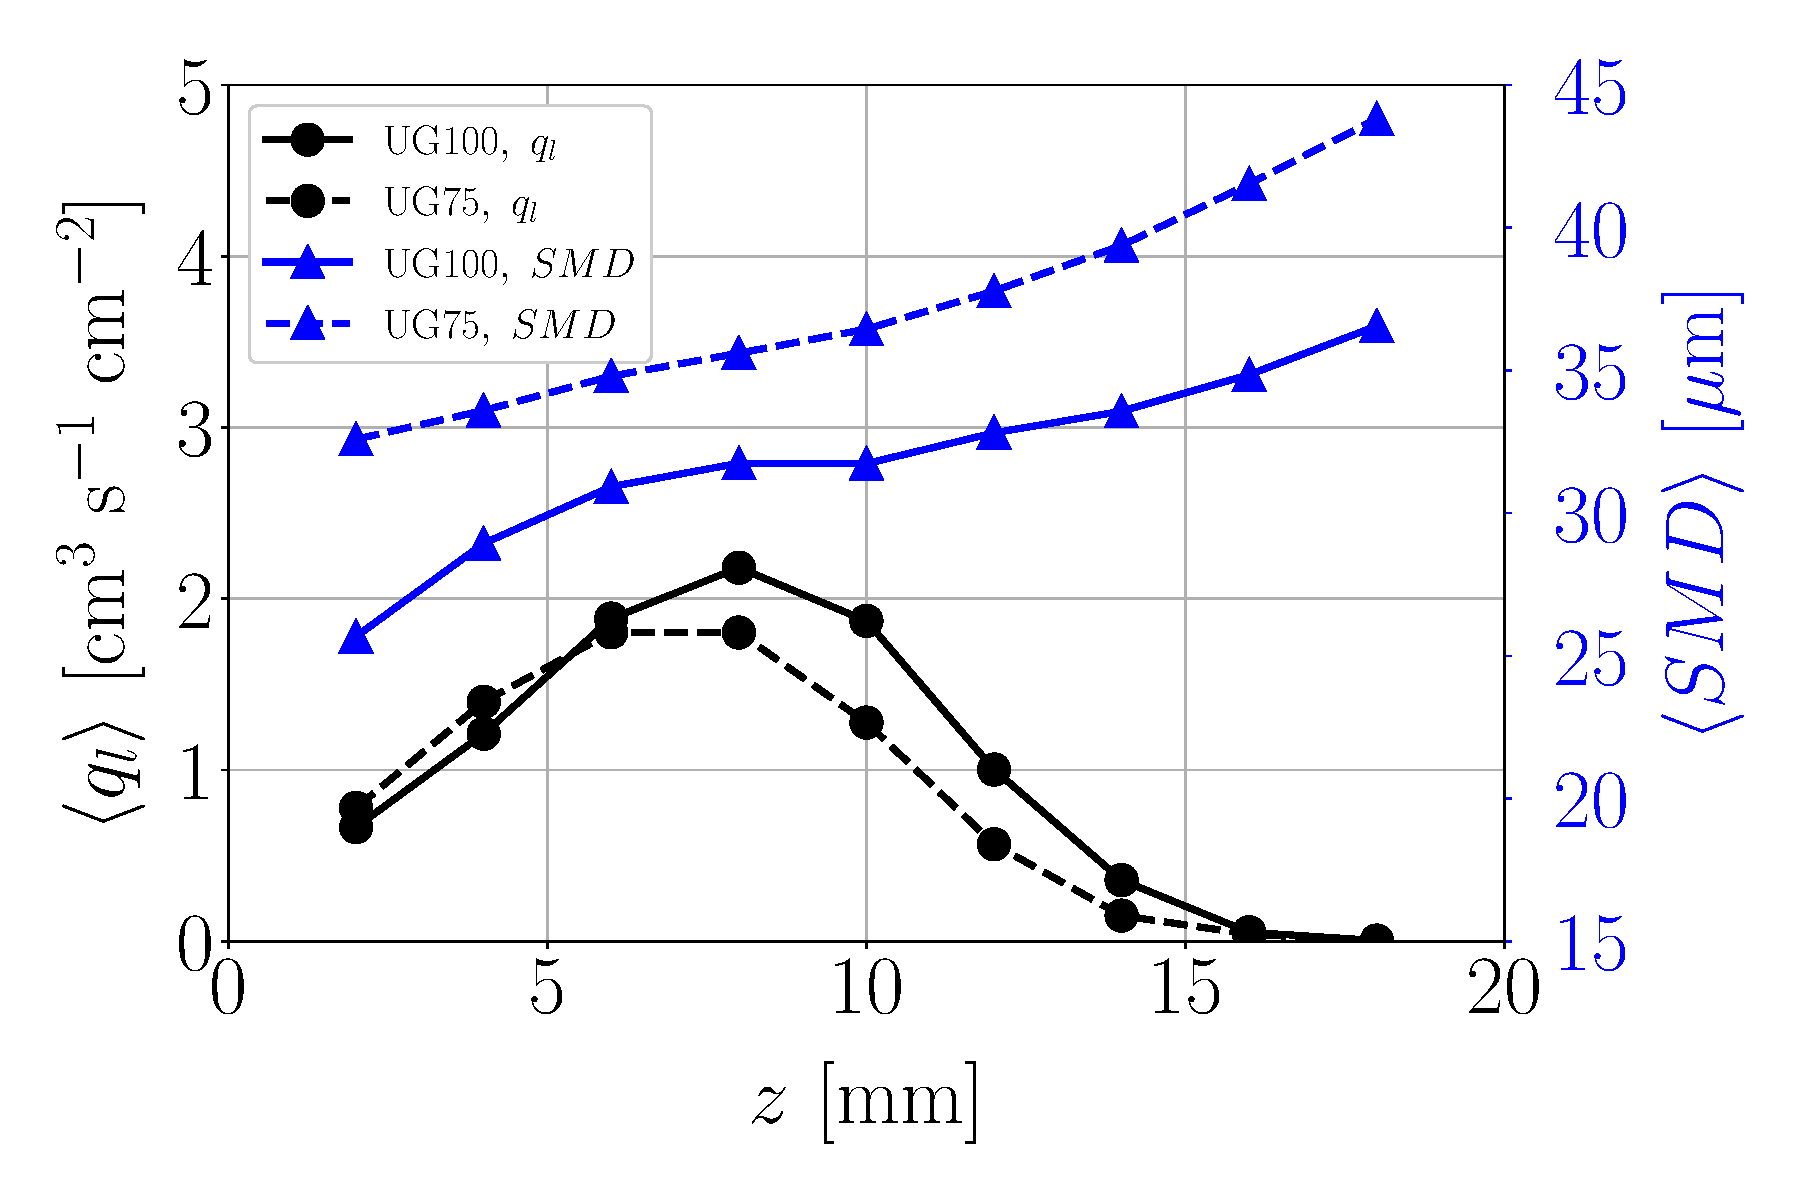
\includegraphics[scale=0.275]{./part2_developments/figures_ch6_lagrangian_JICF/expe_results/integrated_fluxes_along_y}
   \caption{Profiles integrated over $y$.}
  \label{fig:integrated_results_Becker_expe_results_over_y} 
\end{subfigure}
\hspace{0.3in}
\begin{subfigure}[b]{0.45\textwidth}
	\centering
   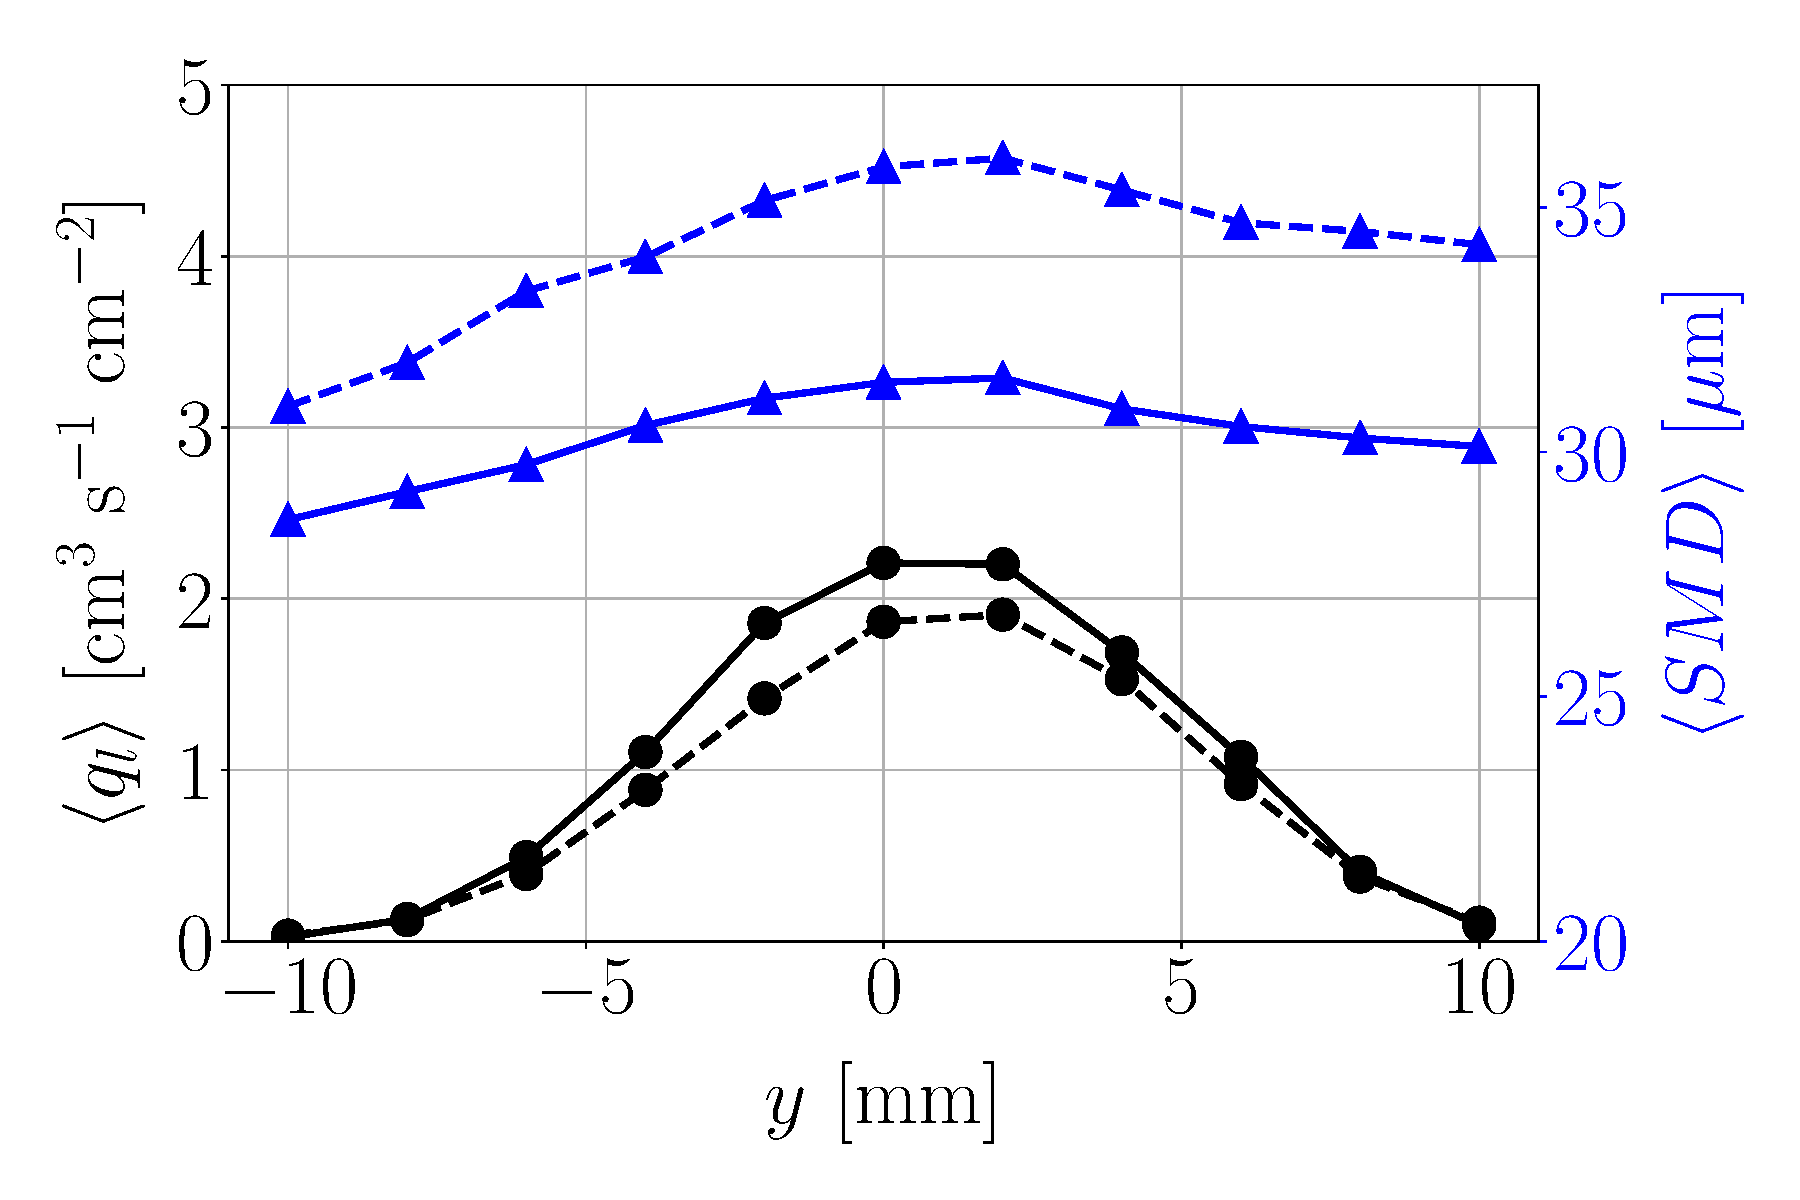
\includegraphics[scale=0.275]{./part2_developments/figures_ch6_lagrangian_JICF/expe_results/integrated_fluxes_along_z}
   \caption{Profiles integrated over $z$.}
  \label{fig:integrated_results_Becker_expe_results_over_z}
\end{subfigure}
\caption[{Integrated liquid volume flux and SMD profiles by \citeColor[becker_breakup_2002] at a location $x = 80$ mm downstream the liquid injector.}]{Integrated liquid volume flux and SMD profiles by \citeColor[becker_breakup_2002] at a location $x = 80$ mm downstream the liquid injector. }
\label{fig:integrated_results_Becker_expe_results}
\end{figure}

\begin{table}[!h]
\centering
\caption{SMDs at $x = 80$ mm obtained from experiments }
\begin{tabular}{cc}
\thickhline
Operating point & $SMD~\left[ \mu \mathrm{m}\right]$  \\
\thickhline
Low Weber & 31.0  \\  
High Weber & 35.2 \\
\thickhline
\end{tabular}
\label{tab:becker_hassa_SMD_values_sprays}
\end{table}


%\section{Sources of uncertainty in PDA measurements}
\section{Uncertainty in experimental data}

The experimental results previously shown, obtained by \citeColor[becker_breakup_2002], were obtained through PDA measurements. PDA is one of the most popular experimental techniques to characterize sprays, since it is non-intrusive and provies information on droplets size and velocities which can then be used to also estimate fluxes. It is not, however, exempt of errors, since it is built on the assumption that droplets are spherical and it is well known that PDA measurements yield considerable erros on droplets sizes and fluxes \citepColor[tropea_optical_2011]. Several sources of error have been identified in the past. \citeColor[bachalo_method_1980] explained that optics play a paramount role: the optical setup can lead to detection errors produced by phenomena associated to the misalignment of dual-beam reflected and refracted rays (Gaussian beam Effect) or to the well-known slit effect, which is cause a truncation on the measurement volume through a slit placed so that the droplet volumes to measure can be defined \citepColor[doublet_effet_2019]. Not associated to the actual setup, modifications in the refractive indices of droplets could affect the scattering and yield important errors in particle sizes, specially relevant in multicomponent fuels such as kerosene. The role of the droplet non-sphericity was discussed, stating that PDA is prone to size overestimation when particles are deformed or oscillate in a preferential direction, as also discussed by \citeColor[damaschke_optical_1998]. \citeColor[dullenkopf_comparative_1998] performed PDA measurements on two injectors, a pressure-swirl and an airblast atomizer, and quantified the errors in mass flux by comparing with the results obtained from a patternator. They identified three main sources of error in the flux estimation: the size measurement (which is powered to 3 to calculate the flux, hence increasing exponentially the flux errors), the number count of droplets and the reference area used for measurements (the smaller the area the better, since it can also avoid counting droplets twice). They found that the flux errors on the pressure swirl fluxes were of the order of 10 $\%$, while in the airblast configurations these increased up to 30 $\%$, and also showed that the SMDs could vary up to 30 $\%$ depending on the PDA system used. \citeColor[brandt_experimental_1998] tested an airblast configuration and discussed several possible sources of error in sizes, highlighting the contribution of alignment uncertainties in the setup ($\sim 1~\%$) the change in refractive indices due to heating ($\sim 3.5~\%$) and to deformation of the sampled particles, since accelerated droplets at high velocity environments will be elliptical rather than spherical and the droplets sizes would be overestimated, propagating later the error to the fluxes calculations (this would explain the larger errors found by \citeColor[dullenkopf_comparative_1998] in their airblast atomizer with respect to the pressure-swirl one). In total, uncertainty on dropsizes was quantified to be of 7 $\%$ while the error on fluxes added up to 10 $\%$ if the particles concentration was not too high. It is worth to remark that the test bench of \citeColor[brandt_experimental_1998] is the same one that \citeColor[becker_breakup_2002] used later at DLR to test the liquid kerosene JICF dealt in this theses (even though the atomizer and the operating conditions are different, the PDA systems and optical configurations are equivalent). The experiments from \citeColor[becker_breakup_2002] do not actually provide data on the dropsize uncertainties, but do discuss the errors on mass fluxes and report mean deviations of 20 $\%$ and maximum of 37 $\%$. A posterior study on this configuration was done by \citeColor[becker_experimental_2004], who tested a swirled injector and reported errors on the SMD of $\sim 5 \%$ (no data on fluxes) attributed to optical misalignment and hardware setting. \citeColor[tropea_optical_2011] makes a review on experimental methods involving optical techniques to characterize disperse multiphase flows, and states that PDA measurements often show uncertainted in flux measurements from $20~\%$ up to several hundrers, while errors in particle size often range, in ideal conditions, from 10 to 30 $\%$. 

The objective here is to estimate possible errors in the experimental measurements of \ref{fig:integrated_results_Becker_expe_results} to obtain confidence intervals for validation of numerical results. As mentioned in the previous paragraph, this study gives a mean uncertainty of 20 $\%$ in the fluxes but does not provide data on the diameters. For the same test bench but with different atomizers and operating conditions, \citeColor[brandt_experimental_1998] reports 7 $\%$ and 14 $\%$ of errors for the droplets diameters and fluxes, respectively, while \citeColor[becker_experimental_2004] give SMD uncertainties of $\sim 5 \%$. Even though the PDA setup is identical in the three studies, the provided errors differ among each other, which might be due to the operating conditions, the atomizer or modifications in the optical setup (indeed, \citeColor[doublet_effet_2019] showed through a error propagation analysis that the uncertainties in the diameters were actually spetially sensitive to the elevation angle of the PDA detectors rather than to other parameters). Therefore, in order to estimate the uncertainty of the diameters in the the experimental setup of \citeColor[becker_breakup_2002], it will be assumed that the relation between the dropsizes and fluxes errors is similar as in the study performed in the same testbench (and in similar operating conditions) by \citeColor[brandt_experimental_1998]: errors between fluxes and diameters differ by a factor of 2, which in case of \citeColor[becker_breakup_2002] yields diameter uncertainties of 10 $\%$ since their mean uncertainty for the fluxes is of 20 $\%$. It is important to keep in mind that this estimated error in droplets size is only approximative and could greatly vary in the actual experiments. \\ %Generally, as shown by the previous literature review,  errors in PDA measurements on droplets sizes are not often reported and characteristic 

Since \citeColor[becker_breakup_2002] give values on the flux uncertainties and their experimental data are available, it is possible to estimate the fluxes obtained from the experiments. The flux map ax $x = 80$ mm for the high Weber operating condition together with the grid composed of the probes through which the spray has been sampled is shown in Figure \ref{tab:previous_numerical_studies_on_jicf_dlr_values}a. Square probes with 2 mm sides are placed as shown in the figure. Each probe contains a volume flux value $q_l$ which is stored atn the center of the probe to plot the maps (\hl{as done in the SLI injectors of Figures \textbf{XX}}). The grid is then composed of $N_y = 11$ probes in the lateral direction and $N_z = 9$ in the vertical one. Given an arbitrary probe located at a position $\left( j,k \right)$ (where $j$ is the probe index in the lateral direction $y$ and $k$ in the vertical one $z$) with surface $S_\mathrm{j,j}$, the absolute liquid flux through this probe can be calculated by applying Eq. (\ref{eq:ch4_volume_flux_definition}) to the probe volume flux $q_{l{j,k}}$:

\begin{equation}
Q_{l_{j,k}} = q_{l_{j,k}} S_{j,k}
\end{equation}

Then, the total liquid flow rate from the map can be calcuated by adding all the absolute fluxes from each probe:

\begin{equation}
Q_{l} = \sum_{j=1}^{N_y} \sum_{k=1}^{N_z} Q_{l_{j,k}} = \sum_{j=1}^{N_y} \sum_{k=1}^{N_z} q_{l_{j,k}} S_{j,k} = 4062 ~ \mathrm{mm}^3~\mathrm{s}^{-1}
\end{equation}

which, as shown, gives a value of $4062 ~ \mathrm{mm}^3~\mathrm{s}^{-1}$. The injected flow rate for this case is $Q_{l,\mathrm{inj}} = 3710~ \mathrm{mm}^3~\mathrm{s}^{-1}$, as given in Table \ref{tab:jicf_operating_conditions}. Therefore, the PDA measurements report a flux excess with respect to the injected flow rate of $9.5~\%$. This deviation is comprised within the mean uncertainty of $20~\%$ provided by the authors of the experiments. Nevertheless, it is paramount to consider this flux overestimation when comparing with the dispersed-phase simulations performed with SLI, since the liquid rates injected in these ones do not correspond to the experimental flux of $4062 ~ \mathrm{mm}^3~\mathrm{s}^{-1}$ but to the injected one of $Q_{l,\mathrm{inj}} = 3710~ \mathrm{mm}^3~\mathrm{s}^{-1}$. In reality, if the PDA was exempt of errors (which, as explained previously, is never the case), the retrieved experimental flux could not be larger than the injected one as mass is not created in the simulation: and actually, it should be lower since there is filming in the experiments, as shown in Figure \ref{fig:jicf_snapshot_expe_filming}, that reduces the liquid flux perpendicular to the crossflow. The resolved simulations could capture this filming phenomenon in the jet, and the filming flux was quantified in $\S$\ref{sec:ch5_direct_measurement_fluxes_IB}.


\begin{figure}[h!]	
	\centering	
	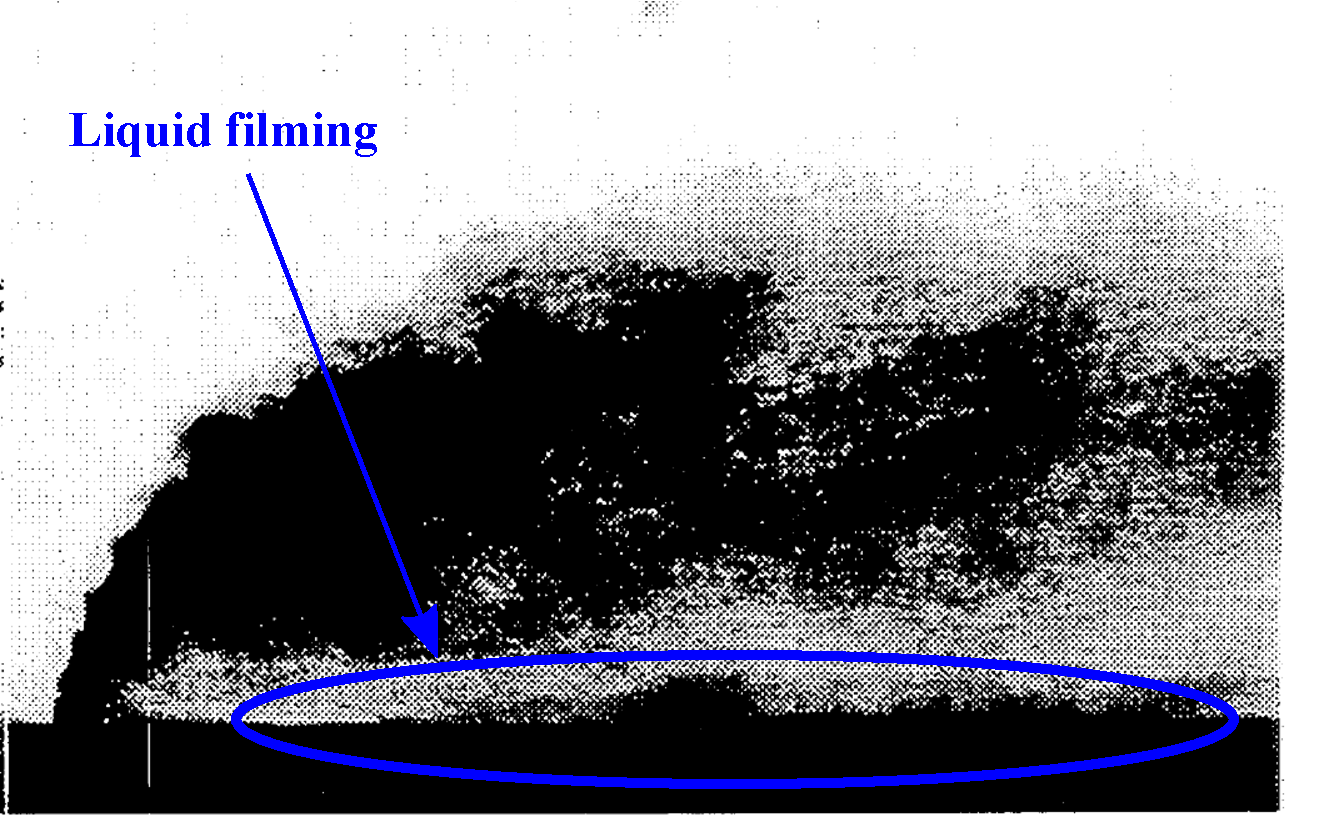
\includegraphics[scale=0.4]{./part2_developments/figures_ch6_lagrangian_JICF/expe_results/snapshot_expe_filming}
	\caption{Snapshot of instantaneous liquid jet from \citeColor[becker_breakup_2002], showing the filming phenomenon}
	\label{fig:jicf_snapshot_expe_filming}
\end{figure}


%snapshot_expe_filming

%\section*{REVIEW on uncertainty: PDA literature}

The work of 1998 paper on ... disclosed errors on the fluxes of 10 $\%$ for a pressure swirl atomizer and of 30 $\%$ for an airblast configuration. Indeed, the experiments of Becker and Hassa report mean errors of 20 $\%$ maximum of 37 $\%$ for liquid fluxes.

PDA present sources of error in:

\begin{itemize}

	\item \textbf{Fluxes}.
	
	\item \textbf{Droplets sizes}. 

\end{itemize}

There are several works that I've obtained dealing with PDA measurement uncertainties. Chronologically:

\begin{itemize}

	\item \textbf{1980 Bachalo} explains that the optical configuration is of particular importance. "\textsl{An error of 10 $\%$ in refractive index results in an error of 10 $\%$ in particle size. For droplets that are deformed in a preferred direction due to, for example, aerodynamic pressure distributions on the droplet, a systematic error in the size measurement could occur}". Hence, if droplets are not spherical the errors can become significant.

	\item \textbf{1998 paper on PDA uncertainties} reports that in previous works (to 1998), errors in fluxes of 100 $\%$ have been reported. Recent efforts (to that date) have been done to minimize such errors. Then, several sources of errors have been identified to arise from the equation used to estimate the flux (put equation somewhere maybe): 1) size measurement due to the third power dependence; 2) umber count depending on the electronics; 3) reference area depending on droplet size, optical configuration and validation scheme. In general, "\textsl{small droplets will not influnce the mass flux significantly so poor detection of small drops should not be a major source of error; however, small droplets sized as large droplets (e.g. slit effect [4]) or large droplets sized as small droplets (trajectory effect [5]) remain problems to be addressed. [...] A final, more subtle, source of error is the alignment and adjustment of the instrument}". This article is also interesting because it compares three different PDA configurations: DualPDA, QS-PDA and PDPA; these are compared to a patternator which is apparently the \textsl{truth}. Two configurations are tested: a pressure-swirl and an airblast atomizer. In general, QS-PDA and DualPDA yield better estimations on the mass fluxes. The pressure-swirl yielded mass flux accuracies of 10 $\%$ for the DualPDA, while the airblast yielded 30 $\%$ (more error).
	
	\item \textbf{1998 Brandt} report how raw PDA data was treated in the same experimental test bench as Becker and Hassa. It is interesting since they test an airblast spray in this configuration. Need to check if the optical setup is exactly the same as in the JICF, but if it is then: \textsl{velocity and dropsize measurement errors due to alignment uncertainties were below 1 \%. Neglecting refractive index gradients, dropsizing errors due to the change of the refractive index of kerosine for droplets being heated up from ambient temperature to their wet-bulb temperature were about 3.5\%}. Errors on droplet diameters are discussed and related to the Bond number (very insteresting), concluding that \textsl{the mean value of the dropsize is measured about 7\% too large.} Later on ($\S$2.3.1), they discuss that volume fluxes errors between 10 and 14 \% were obtained. They also relate errors on sizes due to variations in the refractive index (as in \textbf{1980-Bachalo}). 
	
	\item \textbf{2001 Roisman - Flux measurements ...} develop a model to improve the estimate on size distirbutions and flux measurements with PDA. They emphasize that the difference between detection and illuminated volume is paramount, as well as to consider the error when counting droplets more than one. They also state that PDA errors on \textbf{particles velocities} are not high and they do not affect the fluxes too much: the errors on \textbf{size distributions} are the ones that are important! \textsl{significant sizing errors can be made when the signal-to-noise ratio (SNR) is low or if the premise that a single scattering mode is dominant no longer holds. The latter situation arises via the Gaussian beam effect [2–4] or the slit effect [5]}. To minimize erros, a large enough ratio between diameter of the illuminated volume and the maximum expected particle diameter are chosen. Furthermore, another magnitude susceptible to errors is the \textbf{number of particles} passing through the detection volume during a given observation time. For me, it is necessary to check if the experimental test bench of Becker and Hassa present features that could enhance these errors (the thing on the Brewster's angle might be a clue).

	\item \textbf{2002 Becker}, oh my Goodness how many times I've seen this name, report taht \textsl{at a postion 80 mm downstream the injection point, the difference between measured kerosene mass flows and actualed metered flows was about 20 $\%$ on average, with the maximum difference being 37 $\%$}. 2D-PDA was used: maybe relate it to 1998 article. It is also said that "thereceiving optics could not be positioned at Brewster’s angle (approx. 68 deg) due to limitations of optical access", (ver que demonios es el Brewster angle) which could also affect the results.
	
	\item \textbf{2002 Rachner}, who performed the first computations on this experimental bench, stated that the injected fuel flow rate is not conserved in the measurements at $x = 80$ mm since "\textsl{PDA
measurements are less accurate at high local liquid fluxes because of dense spray effects} (sic)".
	
	\item \textbf{2011 Tropea}
	
	\item \textbf{2016 Eckel} cites \textbf{2011 Tropea} by saying that \textsl{it should be noted that PDA measurements of fuel fluxes are known to have large uncertainties}.
	
	\item \textbf{Malbois 2018 (PhD Thesis)} en verdad no es muy relevante: menciona la PDA brevemente, pero no la utiliza (o no dice utilizarla) y presenta errores en otras medidas.
	
	\item \textbf{Doublet 2020 (PhD Thesis)} si que habla guay de la PDA! Hay que ver la descripcion de la PDA (p. 67) y cuando habla del setup experimental que utiliza (pagina 105), pues aqui hace una propagacion de errores. Igualmente, muestra que la incertitud en los diametros no es muy dependiente de la temperatura, pero MUY dependiente del setup.

\end{itemize}

Also, there are the articles sent by Lea:

\begin{itemize}

	\item \textbf{2004 Becker} (joder con Becker tio) dice que ... Echarle un ojo al correo de Léa, Brunet hace un buen resumen. Igualmente, en el articulo dice que errores de SMD son de un 5 $\%$ (solo?).
	
	\item \textbf{1998 Damaschke} relates that the analysis should depend on the particle types: dependent on shapes, refractive indices, composition and size relative to the wavelength employed. The droplets shapes would affect the light scattering from the particle, which would then affect the measurements.
	
	\item \textbf{1998 Brandt} - Ver arriba.
	
	\item \textbf{2000 Araneo} (careful: diesel spray) quantify the uncertainty in drop diameter and study the influence of the measurement location inside the spray.

\end{itemize}


\section{Previous numerical studies}

Prior to this work, several authors have performed dispersed-phase simulations on the experimental configuration of \citeColor[rachner_modelling_2002]. All cases simulated the high Weber operating point from Table \ref{tab:jicf_operating_conditions}. \citeColor[rachner_modelling_2002] simulated the jet in steady crossflow by considering the early liquid as a cylinder deflected by the airflow, which exchanges momentum with a modified drag coefficient, sheds mass and produces droplets whose properties are given from experimental correlations. Later on, \citeColor[eckel_semi-empirical_2016] extended this model to account for shear breakup of ellipsoids and flattened liquid jets (to account for more realistic JICF dense core effects) in both steady and unsteady crossflows, by using semi-empirical correlations. Independently of these studies, \citeColor[jaegle_large_2009] and \citeColor[senoner_simulation_2010] also developed models with this configuration: the former injected a developed spray at the liquid nozzle while accounting for a modified drag law in the near-nozzle region to mimic the liquid column momentum exchange, and the later injected big blobs at the nozzle but accounting for secondary atomization. All these models (except for
\citeColor[rachner_modelling_2002] since it was more recently improved by \citeColor[eckel_semi-empirical_2016]) are summarized in the diagram of Figure \ref{ch3:subsec_lagrangian_liquid_JICF} and detailed in $\S$\ref{fig:state_art_injection}.

In order to position the current work into the state of the art, it is worth to compare it to the previous studies performed. All the works aforementioned use data shown in Figure \ref{fig:maps_Becker_expe_results} to validate the computations. Nevertheless, not all the numerical studies previously mentioned use all these data for validation, but only display a few of them. Table \ref{tab:previous_numerical_studies_on_jicf_dlr_recap} shows a summary of the validation data directly available in the previous works. None of the papers referred present data on the SMD map, while only \citeColor[eckel_semi-empirical_2016] give data on the global SMD obtained. Most of the works give data on the flux and SMD profiles integrated over $y$, while only \citeColor[rachner_modelling_2002] provides profiles integrated over $y$. %The only work which does not provide data on SMD distributions is \citeColor[eckel_semi-empirical_2016]. 

In first place, the flux maps from all the previous works that provide these information are shown in Figure \ref{fig:maps_previous_numerical_results}. The experimental map is also show for visual comparison. In general, all maps show a circular flux shape and an overestimation of the maximum flux location in the vertical direction (the integrated maps discussed in the following lines confirm this observation). Since the data belonging to the the maps of the numerical studies were unfortunately not directly available, it was obtained by digitalizing the 2D maps depicted in the papers. The grid used for digitalizion is not shown since it was finer than the experimental grid in order to properly capture all the features of the maps, and showing it together with the maps hinders their visualization. From the digitalized maps, the total flux in the plane can be calculated as done previously for the experimental data applying Eq. (\ref{eq:ch6_Ql_total_estimation_from_flux_profiles}). The results are shown in Table \ref{tab:previous_numerical_studies_on_jicf_dlr_values}: even though the fluxes are not exactly equal to the injected flux (the digitalization methodology is not robust enough to retrieve accurately the actual fluxes plotted by the authors, which should be equal to the injected flux and therefore differ from the values obtained), all values are lower than the flux integrated from the experimental map. The only exception is \citeColor[rachner_modelling_2002]: in fact, this work does not display neither maps nor absolute rates, but normalized integrated profiles which in this case have been de-normalized with the injected flux (it has been assumed that the flux retrieved at 80 mm is equal to the injected one). The integrated profiles of the fluxes shown in Figure \ref{fig:previous_works_profiles_comparison_with_expe} confirm these lower flow rates obtained in all simulations performed by each author. These integrated profiles have been obtained through either direct digitalization of the curves when available (Table \ref{tab:previous_numerical_studies_on_jicf_dlr_recap}) or by applying Eq. (\ref{eq:integrated_results_Becker_expe_results}) to the maps when not available. The error bars in the experimental flux profiles of Figure \ref{fig:previous_works_profiles_comparison_with_expe} correspond to a deviation of 20 $\%$ in each point. 


\begin{table}[!h]
\centering
\caption{Available data from previous numerical studies on experimental validation in the configuration of  \citeColor[becker_breakup_2002]}
\begin{tabular}{cccccccc}
\thickhline
\multirow{2}{*}{ Work }  & Global & SMD & Flux & \multirow{2}{*}{ $\langle SMD \left( z \right) \rangle$} & \multirow{2}{*}{ $\langle q_l \left( z \right) \rangle$} & \multirow{2}{*}{ $\langle SMD \left( y \right) \rangle$} & \multirow{2}{*}{ $\langle q_l \left( y \right) \rangle$} \\ 
 & SMD & map & map & & & & \\ 
\thickhline
\citeColor[rachner_modelling_2002] &  & & & \checkmark & \checkmark & \checkmark & \checkmark \\
\citeColor[jaegle_large_2009] & & & \checkmark & \checkmark & \checkmark & & \\
\citeColor[senoner_simulation_2010] & & & \checkmark & \checkmark & \checkmark & & \\
\citeColor[eckel_semi-empirical_2016] & \checkmark & & \checkmark & & & & \\
\thickhline
\end{tabular}
\label{tab:previous_numerical_studies_on_jicf_dlr_recap}
\end{table}

\begin{figure}[h!]
\flushleft
\begin{subfigure}[b]{0.2\textwidth}
	\flushleft
%	\hspace*{-0.35in}
   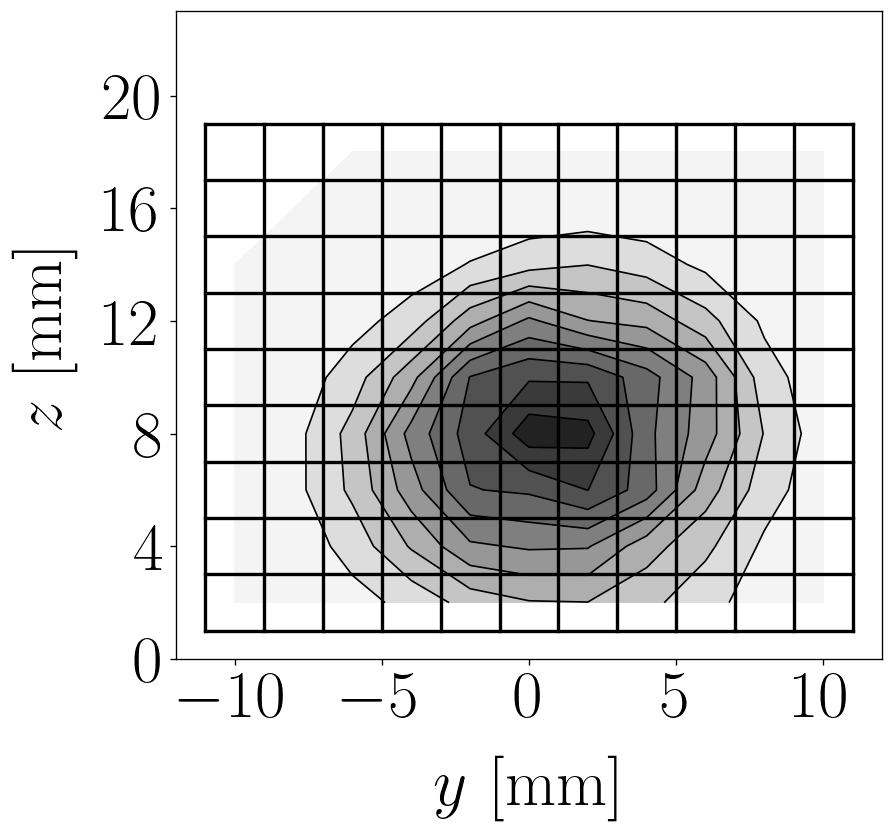
\includegraphics[scale=0.225]{./part2_developments/figures_ch6_lagrangian_JICF/previous_numerical_results/map_expe}
   \caption*{\hspace{0.35in}(a) Experimental}
   %\label{} 
\end{subfigure}
\hspace*{0.35in}
\begin{subfigure}[b]{0.2\textwidth}
	\flushleft
   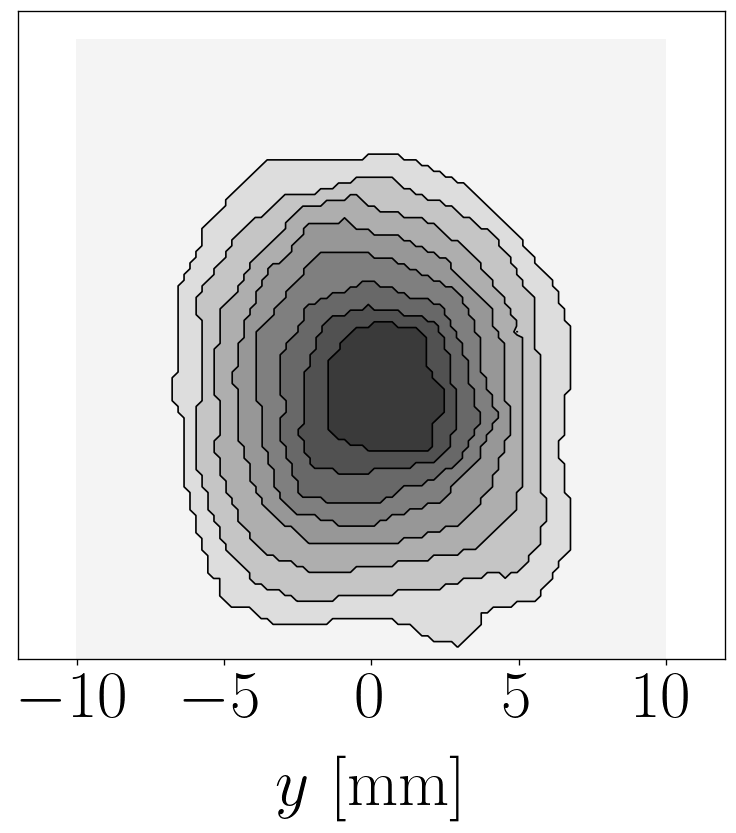
\includegraphics[scale=0.225]{./part2_developments/figures_ch6_lagrangian_JICF/previous_numerical_results/map_jaegle}
   \caption*{(b) Jaegle (2009)}
   %\label{} 
\end{subfigure}
\hspace*{0.05in}
\begin{subfigure}[b]{0.2\textwidth}
	\flushleft
   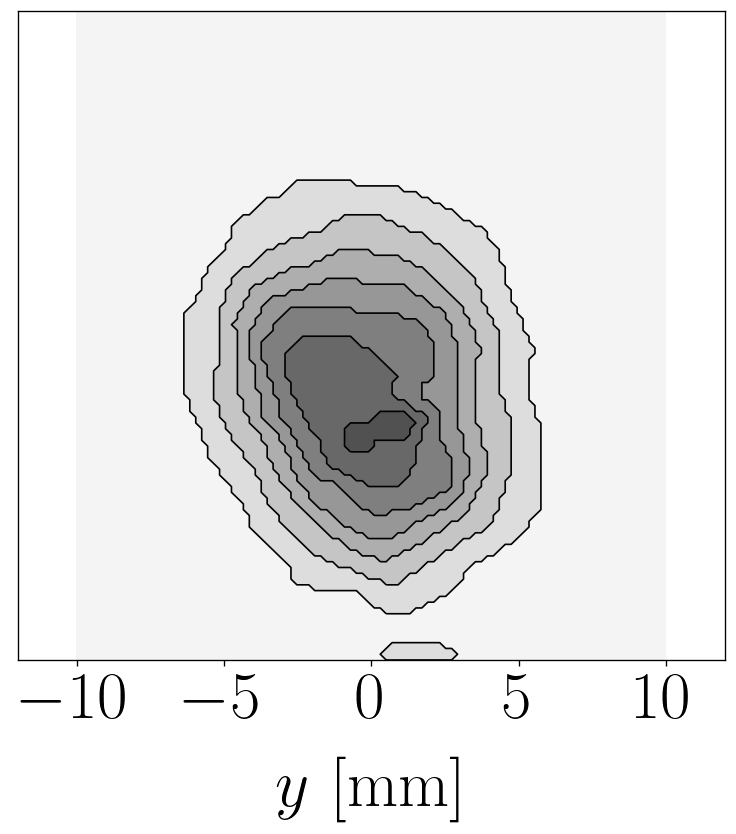
\includegraphics[scale=0.225]{./part2_developments/figures_ch6_lagrangian_JICF/previous_numerical_results/map_senoner}
   \caption*{(c) Senoner (2010)}
   %\label{} 
\end{subfigure}
\hspace*{0.05in}
\begin{subfigure}[b]{0.2\textwidth}
	\flushleft
   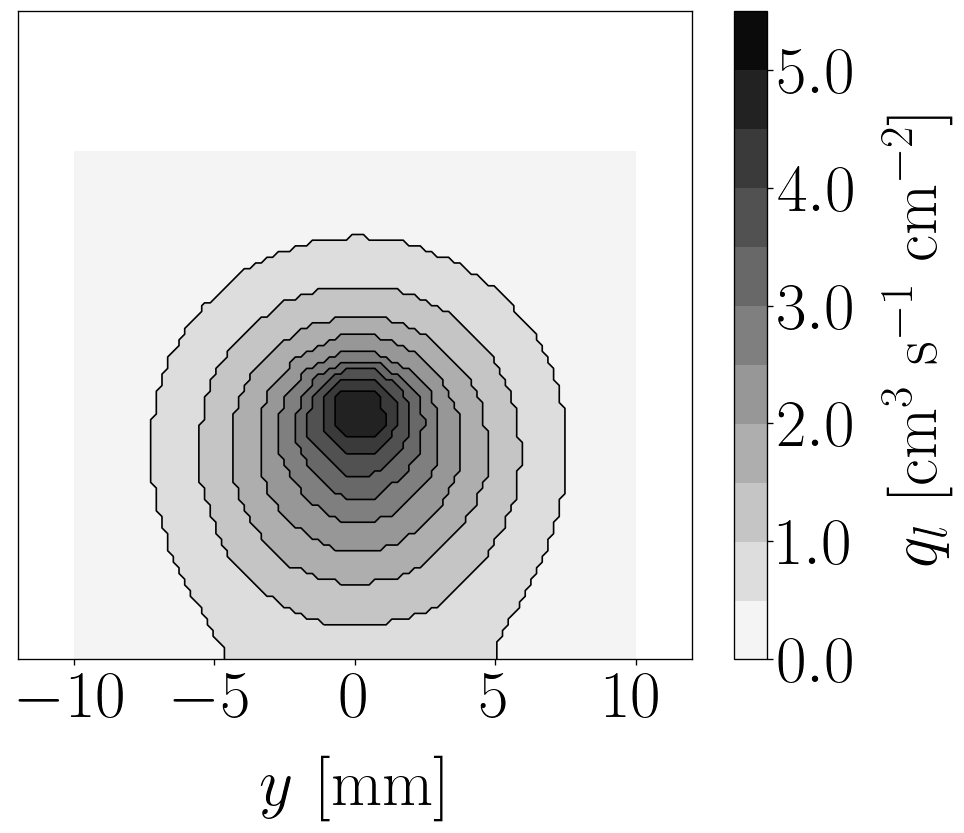
\includegraphics[scale=0.225]{./part2_developments/figures_ch6_lagrangian_JICF/previous_numerical_results/map_eckel}
   \caption*{(c) Eckel (2016)}
   %\label{} 
\end{subfigure}
\caption{Volume flux maps at $x = 80$ mm obtained for the high Weber operating conditions from experiments \citepColor[becker_breakup_2002] and past computational works on the same configuration and operating condition. The experimental map shows the grid composed of the probes through which the spray is characterized}
\label{fig:maps_previous_numerical_results}
\end{figure}

As previously mentioned, none of the previous works display SMD maps. Most of the works report, on the other hand, $SMD$ integrated profiles over $y$: these have been digitalized and are shown in Figure \ref{fig:previous_works_profiles_comparison_with_expe}.   The error bars in the experimental SMD profiles at this Figure correspond to a deviation of 10 $\%$ in each point. All cases show a ballistic behaviour in which the SMD increases with vertical distance $z$. The SMD profiles integrate over $z$ are only present in \citeColor[rachner_modelling_2002], who obtained accurate results at the center of the spray (region of maximum flux location) and showed a SMD overestimation when moving away towards the edges.

From the SMD integrated profiles over $y$, a global SMD can be estimated by performing a further integration along the $z$ direction:

\begin{equation}
 SMD =  \frac{1}{ \int_0^{L_z} \langle q_l \left( z \right) \rangle dz} \int_0^{L_z} \langle q_l \left( z \right) \rangle \langle SMD \left( z \right) \rangle dz
\end{equation}


Results are shown in Table \ref{tab:previous_numerical_studies_on_jicf_dlr_values}.  \citeColor[eckel_semi-empirical_2016] do not provide the integrated SMD profile, yet they give directly the global SMD. Generally, all SMDs show a good agreement with respect to the experimental value of \citeColor[becker_breakup_2002]. The works of \citeColor[rachner_modelling_2002] and \citeColor[eckel_semi-empirical_2016] perform a calibration of their model to match the experimental size distribution, hence such a good agreement is expected. Similar is the case of \citeColor[jaegle_large_2009], who already injected the experimental size distribution at the injector without including any secondary atomization model: then, the flux-weighted SMD is expected to be close to the SMD of this distribution. \citeColor[senoner_simulation_2010] does not inject any distribution but injects droplets at the liquid nozzle with size equal to the nozzle's diameter, drags them with a modified momentum transfer law at the column liquid region and then applies the stochastic secondary breakup model of \citeColor[gorokhovski_stochastic_2001], used in this thesis and explained in $\S$\ref{subsec:ch4_goro_model}, to account for further breakup of droplets. The good results in terms of global SMD and integrated profiles obtained in his work denote the suitabitliy of the stochastic breakup model to simulate such configurations.




%\citeColor[rachner_modelling_2002], who performed the first computations on this experimental bench, stated that the injected fuel flow rate is not conserved in the measurements at $x = 80$ mm since "\textsl{PDA measurements are less accurate at high local liquid fluxes because of dense spray effects} (sic)". \hl{...} The experimental volume flux map at $x = 80$ together with the grid in whose center the measurement probes have been located is shown in Figure \hl{\textbf{XX}} left. For each discrete probe ($j,k$), the absolute flux $Q_{l_{j,k}}$ can be calculated as:


\begin{figure}[h!]
\flushleft
\begin{subfigure}[b]{0.9\textwidth}
	\centering
   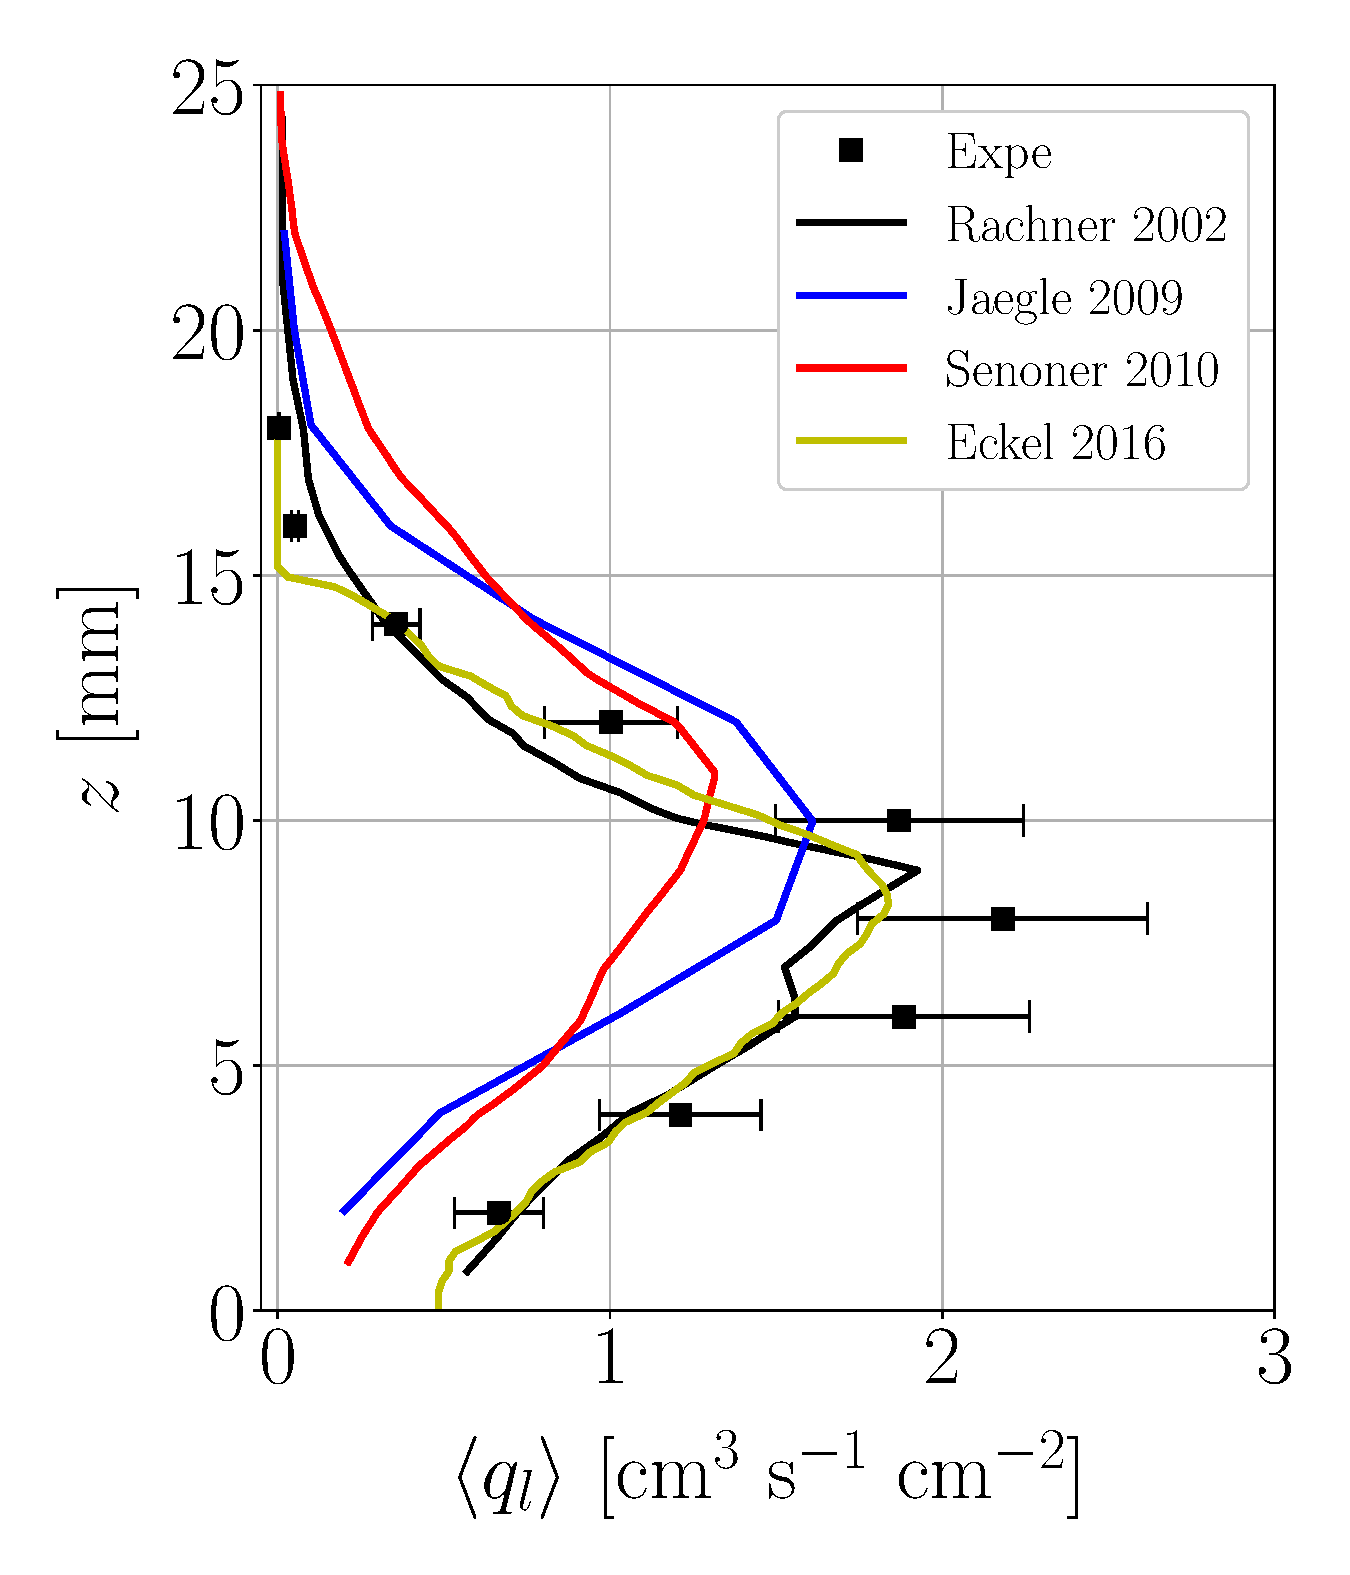
\includegraphics[scale=0.22]{./part2_developments/figures_ch6_lagrangian_JICF/previous_numerical_results/flux_profiles_along_z}
%    \hfill
   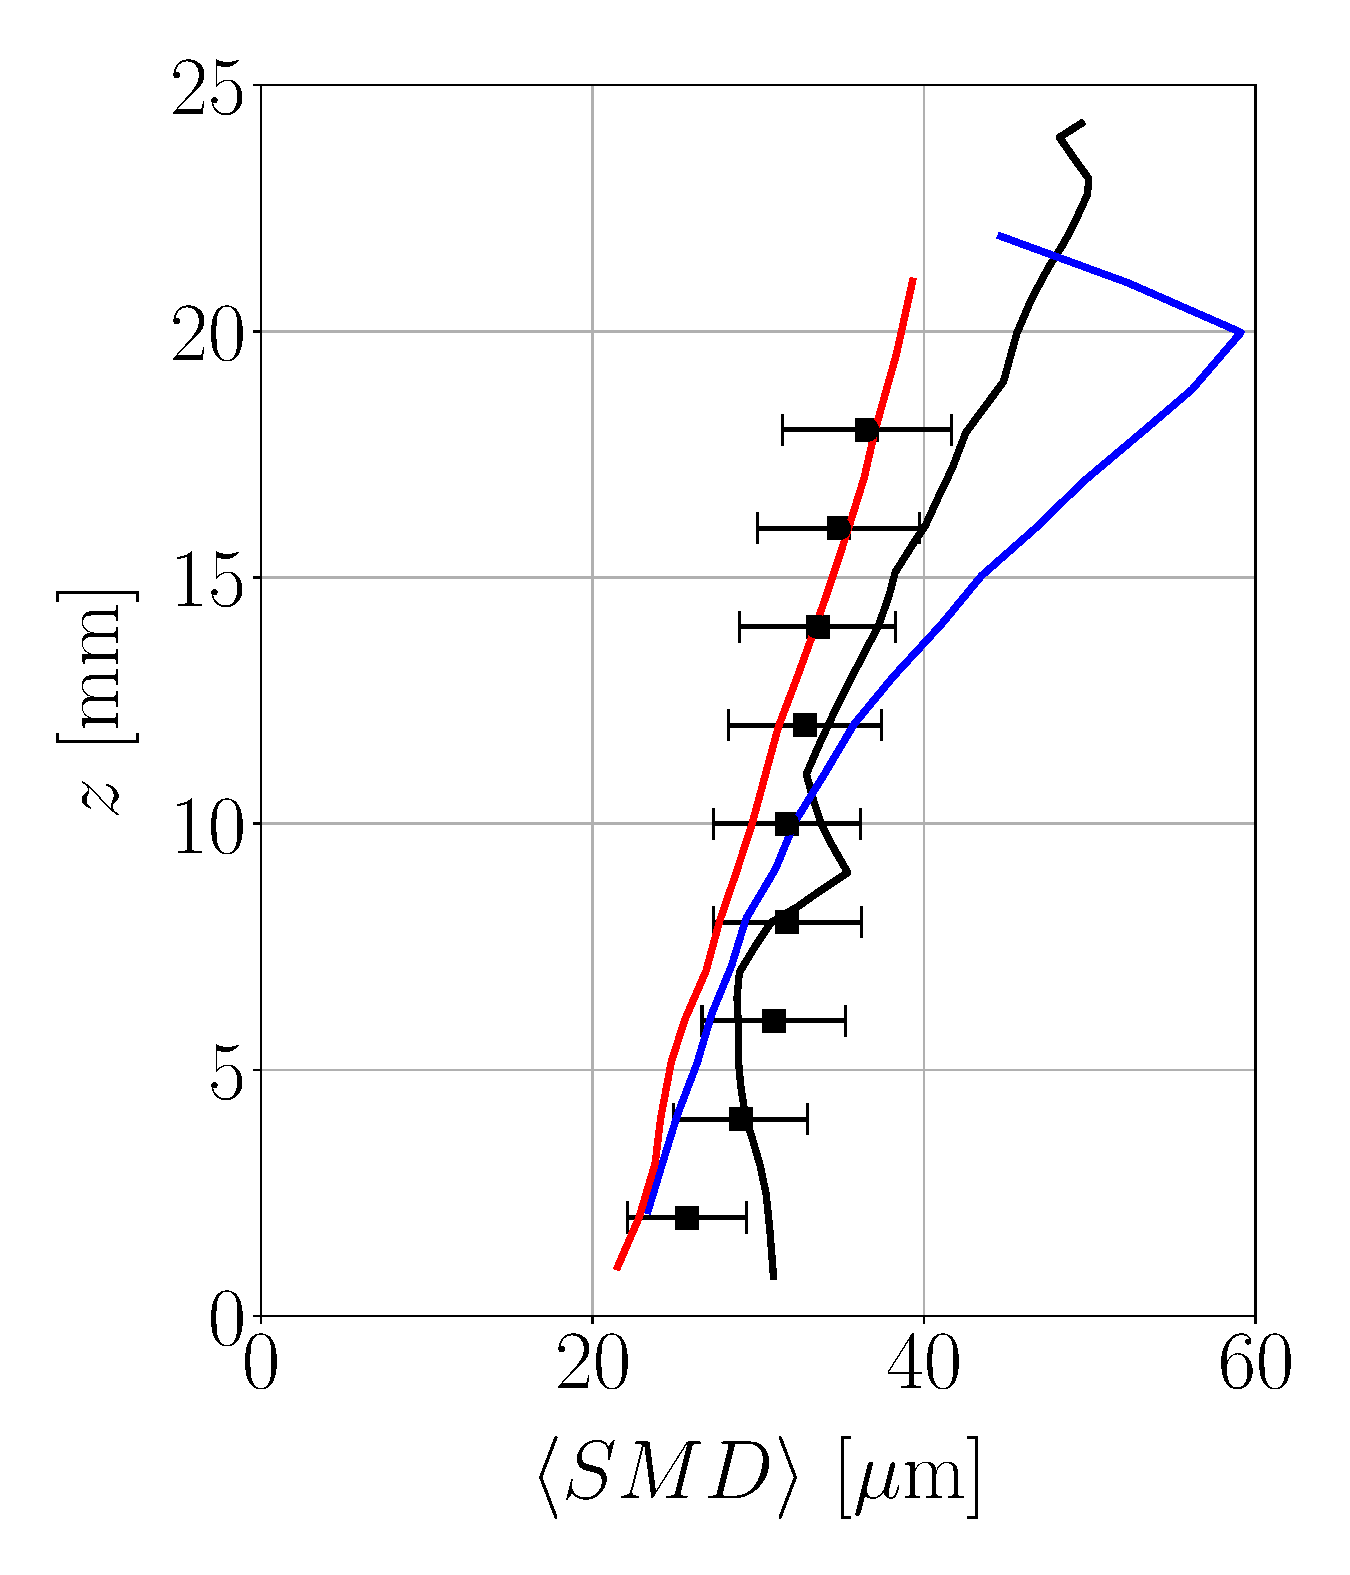
\includegraphics[scale=0.22]{./part2_developments/figures_ch6_lagrangian_JICF/previous_numerical_results/SMD_profiles_along_z}
   \caption{Profiles integrated over y}
   %\label{} 
\end{subfigure}

\vskip\baselineskip

\begin{subfigure}[b]{0.9\textwidth}
	\centering
   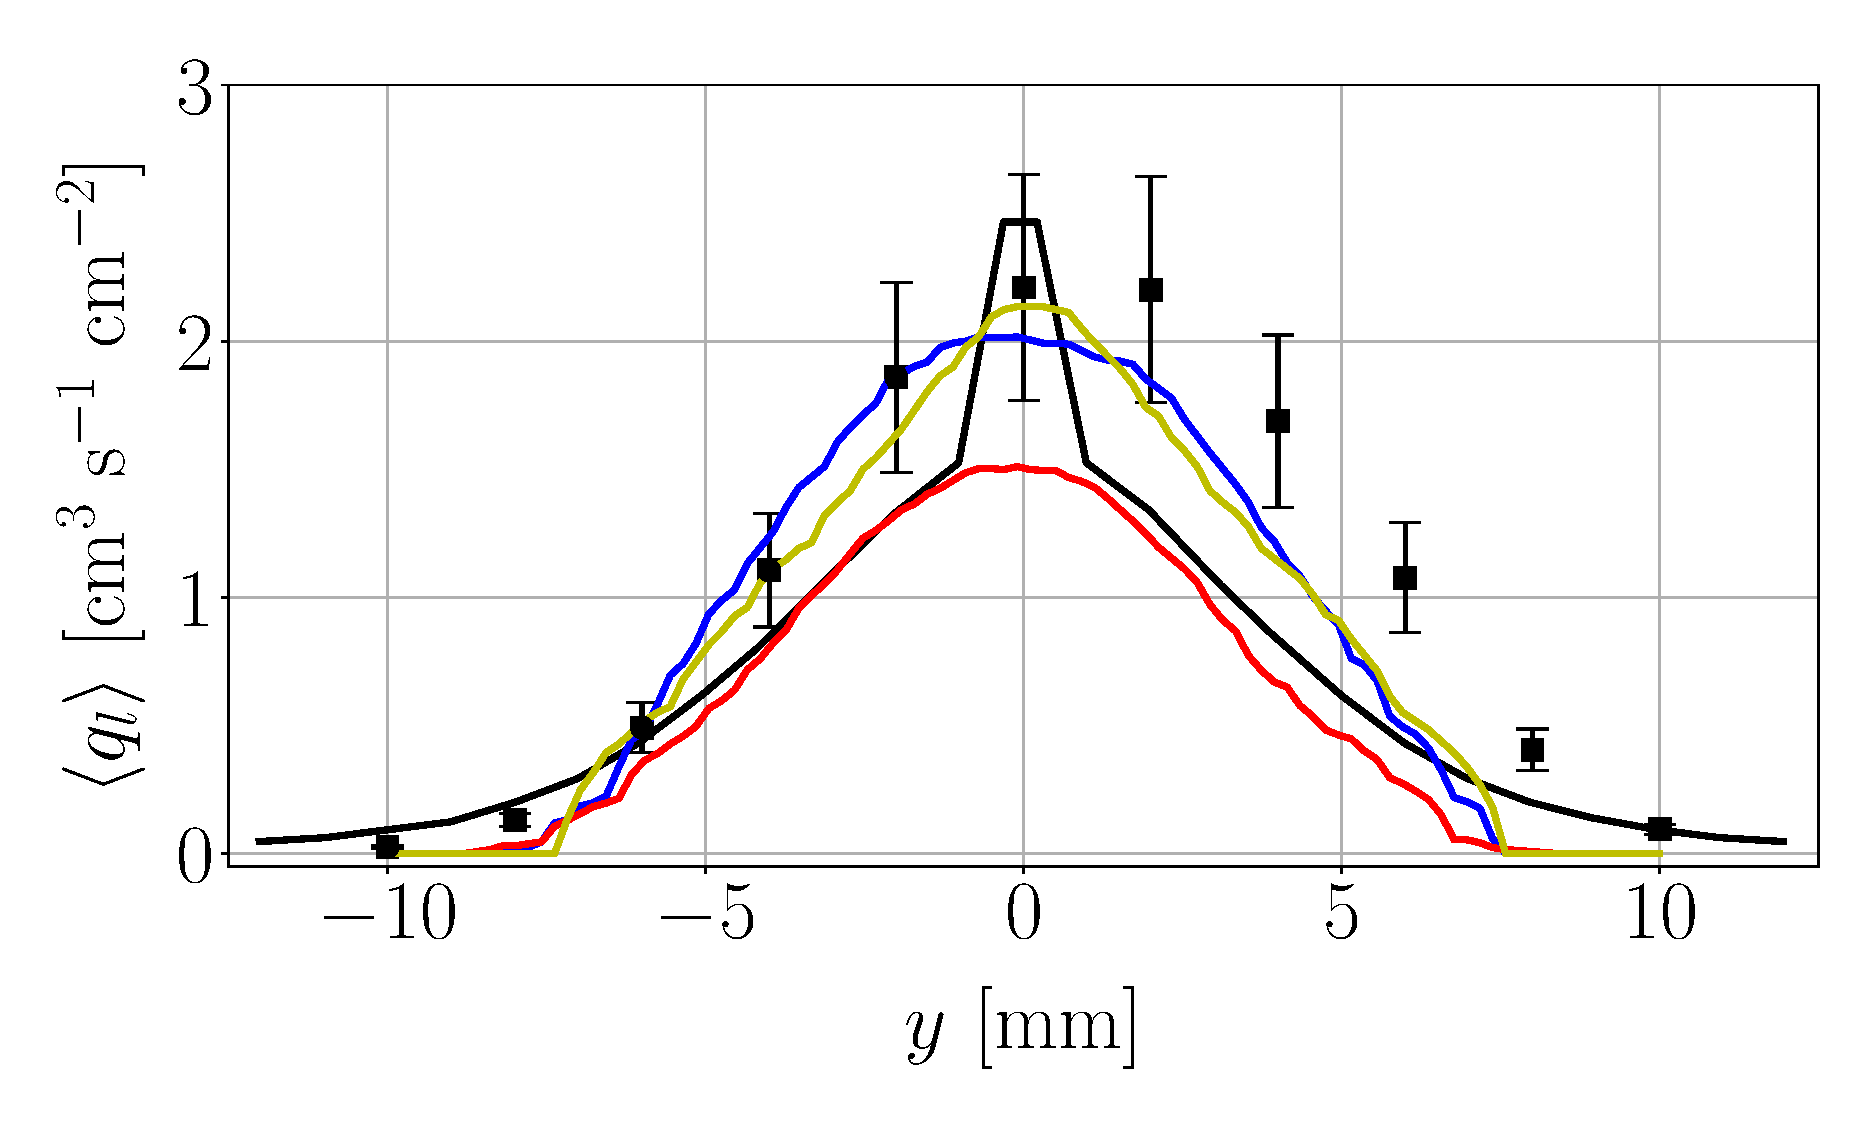
\includegraphics[scale=0.22]{./part2_developments/figures_ch6_lagrangian_JICF/previous_numerical_results/flux_profiles_along_y}
    %\hfill
   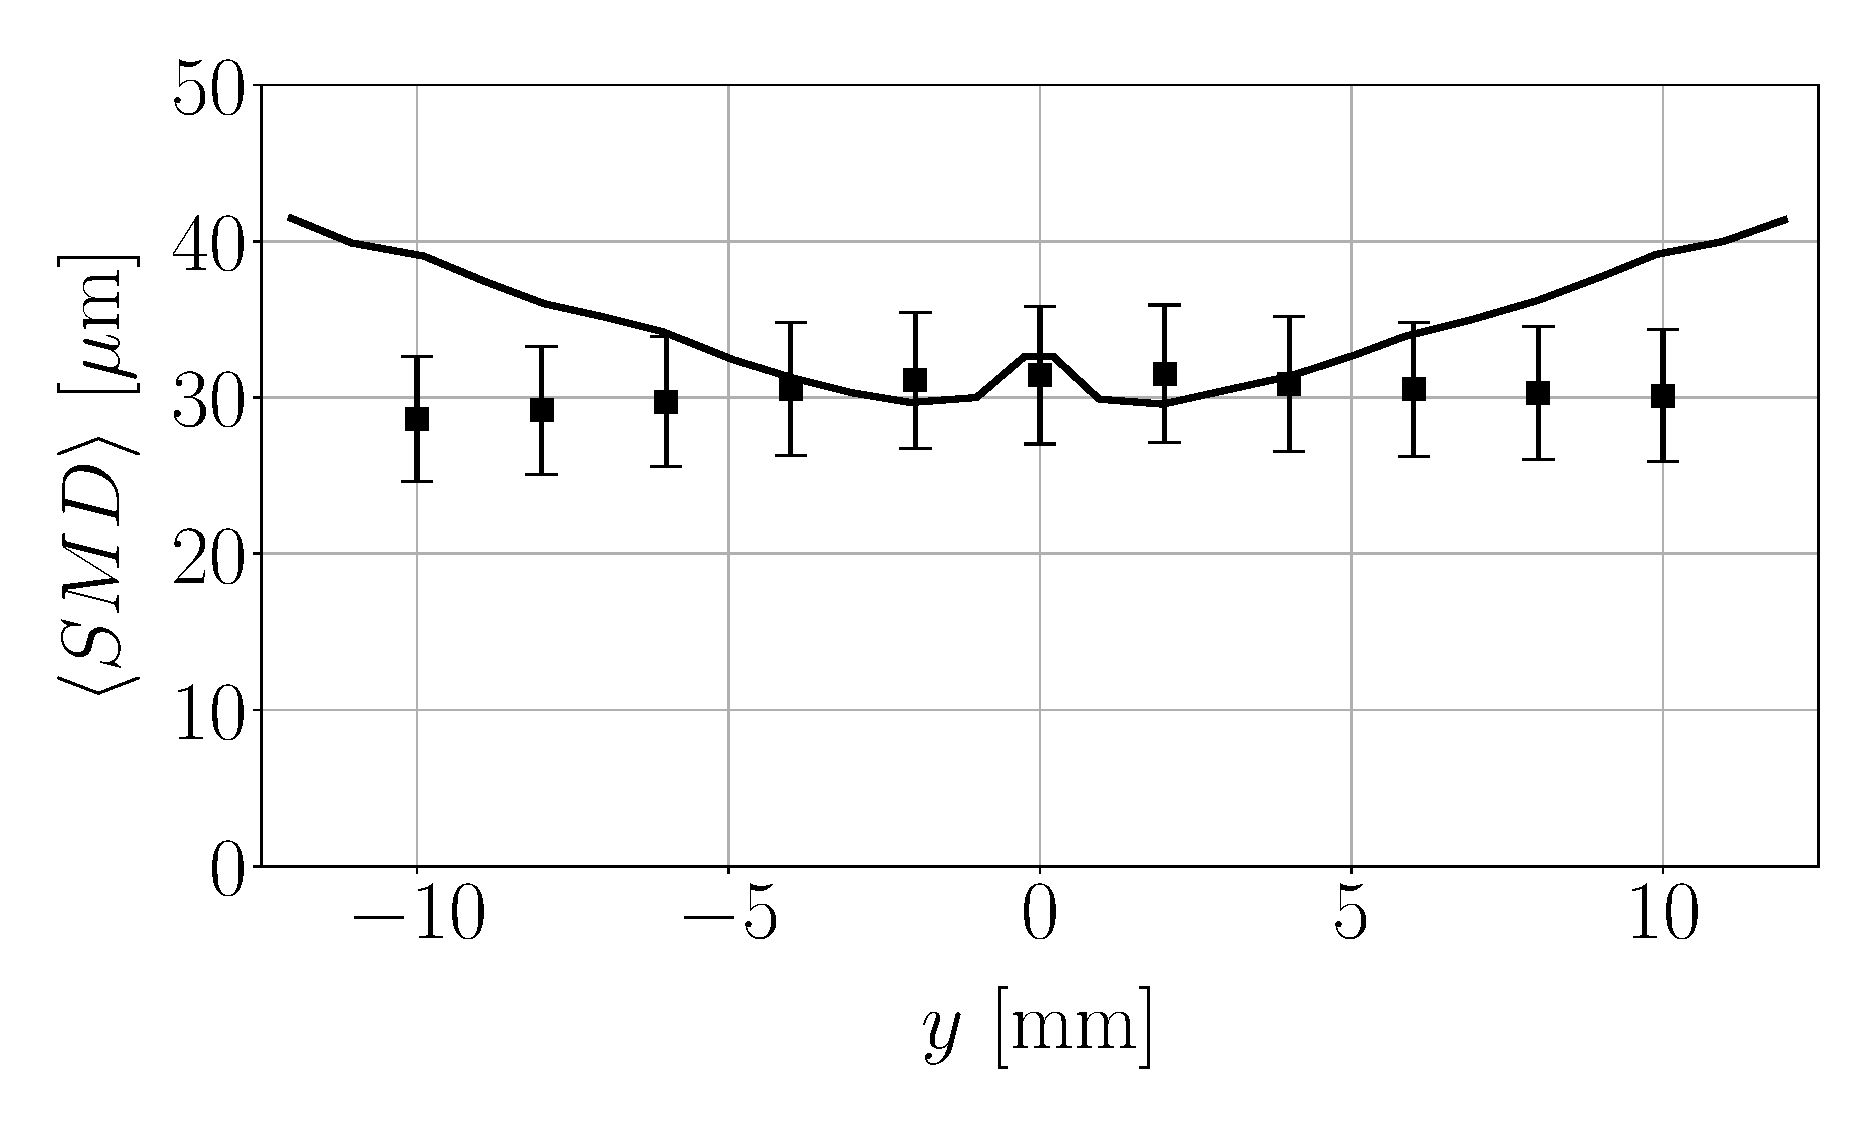
\includegraphics[scale=0.22]{./part2_developments/figures_ch6_lagrangian_JICF/previous_numerical_results/SMD_profiles_along_y}
   \caption{Profiles integrated over z}
   %\label{} 
\end{subfigure}
\caption{Integrated $SMD$ and volume flux profiles from experiments and past computational works. Computational fluxes have been obtained through digitalization and are hence not fully reliable }
\label{fig:previous_works_profiles_comparison_with_expe}
\end{figure}

\clearpage

\begin{table}[!h]
\centering
\caption{Global data obtained at $x = 80$ mm from experiments and previous computational studies }
\begin{tabular}{ccc}
\thickhline
Reference & $SMD~\left[ \mu \mathrm{m}\right]$  & $Q_l~\left[ \mathrm{mm}^3 s^{-1} \right]$ \\
\thickhline
\citeColor[becker_breakup_2002] & 31.0 &   4062  \\  
\citeColor[rachner_modelling_2002] & 31.9  & 3710  \\
\citeColor[jaegle_large_2009] & 33.2 &  3693.8  \\
\citeColor[senoner_simulation_2010] & 29.6  & 3573  \\
\citeColor[eckel_semi-empirical_2016] & 32.7  & 3775.9  \\
\thickhline
\end{tabular}
\label{tab:previous_numerical_studies_on_jicf_dlr_values}
\end{table}


%\begin{table}[!h]
%\centering
%\caption{Data obtained from previous work }
%\begin{tabular}{ccccc}
%\thickhline
%Work & $SMD~\left[ \mu \mathrm{m}\right]$ & $\varepsilon_{SMD}~\left[\% \right]$ & $Q_l~\left[ \mathrm{mm}^3 s^{-1} \right]$ & $\varepsilon_{Q_l}~\left[ \% \right]$ \\
%\thickhline
%\citeColor[becker_breakup_2002] & 31 & &  4062&  \\  
%\citeColor[rachner_modelling_2002] & 31.9 & & 3710 & \\
%\citeColor[jaegle_large_2009] & 33.2 & & 3693.8 & \\
%\citeColor[senoner_simulation_2010] & 29.6 & & 3573 & \\
%\citeColor[eckel_semi-empirical_2016] & 32. & & 3775.9 & \\
%\thickhline
%\end{tabular}
%\label{tab:previous_numerical_studies_on_jicf_dlr_values}
%\end{table}




\section{Obtention of boundary conditions for gaseous phase}
\label{sec:ch6_BC_gaseous_phase}

Prior to liquid injection, it is necessary to establish an initial solution for the gaseous phase as done for the resolved simulations. The difference with respect to the resolved simulations is that in this case, the initial solutions needs to consider the ALM since the dense core blockage effect needs to be modelled in the dispersed phase simulations. All the details of the model were addressed in $\S$\ref{sec:ch4_dense_core_modelling}. In this section, results from the resolved simulations are employed as input parameters to feed the ALM model. It is shown that the initial parameters do not capture correctly the gaseous turbulent structures, and are tuned in order to find an optimal configuration that better retrieves them. This optimal configuration is nevertheless not able to capture all the gaseous features, and another methodology to prescribe inlet boundary conditions obtained from the resolved atomization simulations in a reduced computational domain.


\subsection{Actuator Line Model}

%\subsection{Setup of actuator model}

The model parameters for ALM were described in Table \ref{tab:alm_parameters}. For the two operating points simulated, the corresponding input parameters are summarized in Table \ref{tab:jicf_lgs_ALM_parameters}. These parameters are 

The final actuator point $x_b$, $z_b$ and $c_L$ are obtained from the mean values of Figure \ref{fig:dense_core_mean_parameters_scatterplots} for the fine simulations (note that $c_L$ is equivalent to the resolved dense core width $w$); $c_0$ is equal to the injector diameter; $N_p$ has been set to 20 as default, but it has been checked not to have an effect on the results; and the force $\textbf{F}_\mathrm{DC}$ is obtained as explained in $\S$\ref{ch5:subsec_defining_pressure_differences}.

\begin{table}[!h]
\centering
\caption{Parameters of an actuator representing the dense core for the high Weber case}
\begin{tabular}{cccc}
\thickhline
\textbf{Parameter} & \textbf{Units} & \textbf{Initial} &  \textbf{Final} \\
\thickhline
$x_b$ & mm & & \\
$z_b$ & mm & & \\
$c_0$ & mm & 0.45 & 0.45 \\
$c_L$ & mm & & \\
$| \textbf{F}_\mathrm{DC} |$ & N &  & \\
%$\Delta p$ & Pa &  & \\
\thickhline
\end{tabular}
\label{tab:jicf_lgs_ALM_parameters}
\end{table}

An example of an actuator representing the dense core in gaseous simulations \hl{can be seen in Figure }. As observed, it is graphically represented as a cylinder with the initial point located in the injection nozzle exit and final point in the breakup location of the resolved dense core estimated from the resolved simulations. The actuator points (not shown in the figure) are located uniformly along the central line of the cylinder. The discrete forces applied to each point are then mollified in the neighbouring cells in order to avoid flow singularities.

\subsubsection{Comparison between resolved and ALM gaseous fields}

The perturbed gaseous fields created by the presence of the dense core in the \hl{resolved simulations were discussed in $\S$}\ref{ch5:subsec_turbulent_structures_in_gaseous_field}. In the same fashion, equivalent postprocessings can be performed for the gaseous flow field 

A quantitative assessment of the actuator blockage effect can be performed by looking at the mean velocity distribution along the lines \textbf{XX} shown in Figure \ref{XX}. Equivalent data was obtained for the resolved simulations in \hl{\textbf{$\S$XX}}, which is also shown in the same Figure for comparison ... \\


\subsubsection{Parametric study on actuator model}


\subsection{Prescription of gaseous inlet from resolved simulations }


\subsubsection{Methodology}

As previously shown, the ALM model has been proved to be able to perturb the gaseous field. \hl{From an initial actuator obtained from the parameters of the resolved atomization simulation, the forces have been tuned to seek for a better match of the mean velocity profiles in the dispersed-phase simulations}. The match, however, is not completely accurate and the perturbation effect from the resolved simulations cannot be fully captured by ALM, since the dynamics and topology of the liquid dense core hinder their modelling with the relatively simple ALM model developed. 

With the objective of trying to improve the matching of the resolvded gaseous fields, a different strategy has been approached. This one is based on obtaining the gaseous field in a plane perpendicular to the crossflow from the resolved simulations. The field is characterized by the mean and RMS values of the velocities in the three directions. Such profiles are then imposed in a reduced domain consisting of a box with length $150$ mm and cross-section 25x40 mm$^2$ representing the downstream part of the plenum from the JICF configuration of Figure \ref{fig:numerical_setup_maquette_JICF_DLR}. A schematic of the methodology is illustrated in Figure \ref{fig:custom_inlet_methodology}. The velocity profiles are imposed at the inlet of the prescribed domain according to the following law:

\begin{equation}
\textbf{u} \left( \textbf{x}, t \right) = \overline{\textbf{u}} \left( \textbf{x} \right)  + r \left( t \right)  \textbf{u}_\mathrm{RMS} \left( \textbf{x} \right) 
\end{equation}

where $\overline{\textbf{u}} \left( \textbf{x} \right)$ and $\textbf{u}_\mathrm{RMS} \left( \textbf{x} \right)$ are the mean and RMS velocity distributions in the crossflow plane extracted from the resolved atomization simulations. $r \left( t \right)$ is a time-varying scalar sampled from a normal distribution with mean 0 and variance 1: $r \sim \mathcal{N} \left( \mu = 0, \sigma^2 = 1 \right)$. This velocity prescription law, which is based on the weak recycling method of synthetic turbulence injection by \citeColor[wu_large_1995], ensures that the injected $TKE$ in the dispersed phase simulations is the same as the one retrieved from the resolved atomization ones. \hl{Nevertheless, due to the coarser mesh employed in the reduced domain with respect to the }

\begin{figure}[h!]	
	\centering	\includeinkscape[inkscapelatex=false,scale=0.25]{./part2_developments/figures_ch6_lagrangian_JICF/gas_field_initial_conditions/custom_inlet_methodology}
	\caption{Methodology to prescribe mean and RMS velocity fields from resolved simulations in reduced domain for dispersed-phase computation.}
	\label{fig:custom_inlet_methodology}
\end{figure}

The mesh employed for performing simulations with the prescribed inlet is shown in Figure \ref{fig:mesh_reduced_inlet}. The mesh, which contains $12 \cdot 10^6$ elements, has been refined up to a location $x = 40$ mm downstream the inlet to a mesh size $\Delta x = 0.3$ mm, while from $x = 40$ mm up to $x = 100$ mm, the mesh size has been set to $\Delta x = 0.5$ mm as in the mesh of Figure \ref{fig:jicf_dlr_mesh_LGS}. The finer cell size of $\Delta x = 0.3$ mm has been selected  with the objective of better capturing the turbulent structures created by the inhomogeneous gaseous velocity profile injected. Nevertheless, \hl{as it will be shown later}, this cell size is not resolved enough to capture those: in the resolved simulations of Chapter \ref{ch5:jicf_resolved_simulations}, the cell size in the gaseous field around the liquid regions was of the order of the interface cell sizes ($20, 10~\mu$m) created by the ALM method, while such resolutions cannot be imposed into this reduced domain as the mesh size greatly increases and yields computations considerably expensive. Furthermore, a too fine mesh would create large volume fractions which are not in accordance with the application of lagrangian methods to simulate dispersed multiphase flows, which are applicable to small volume fractions \citepColor[murrone_numerical_2011].

\begin{figure}[h!]	
	\centering	
	\includeinkscape[inkscapelatex=false,scale=0.4]{./part2_developments/figures_ch6_lagrangian_JICF/mesh_reduced_inlet}
	\caption{Mesh used for a direct prescription of velocity profiles at gaseous inlet in dispersed-phase simulations}
	\label{fig:mesh_reduced_inlet}
\end{figure}



\subsubsection{Setup and results}

The injected profiles, shown in the maps of Figure \ref{fig:custom_inlet_methodology}, have been obtained from the location $x = 3$ mm downstream the liquid injector in the resolved atomization simulations. Other plane locations have been tested without observing significant differences in the velocity profiles in the dispersed-phase simulations. In fact, the range of the possible planes to retrieve gaseous data for prescribing inlet BCs is narrow: upstream $x = 3$ mm the jet dense core is present and mean gaseous profiles would contain velocities corresponding to the liquid phase, while further downstream the lagrangian spray is injected in the dispersed-phase simulations (the earliest injection location is $x = 5$ mm). Hence, the only reported case here corresponds to the location $x = 3$ mm. Since the computational domain is reduced with respect to the full computational configuration used for the ALM, the axial coordinates are shifted 3 mm and the experimental validation plane, located at 80 mm downstream the liquid injection nozzle in the test bench, corresponds to the location $x = 77$ mm as depicted in Figure \ref{fig:mesh_reduced_inlet}. Hereafter, however, all axial coordinates reported will be expressed in the absolute reference frame of the experimental test bench for easening comparison with the ALM dispersed-phase simulations.



\subsection{Comparison between ALM and prescribed gas profiles}

Planes y in Figure \ref{fig:JICF_lgs_gaseous_conditions_comparison_plane_y}. Planes x in Figure \ref{fig:JICF_lgs_gaseous_conditions_comparison_planes_x}. 

\begin{figure}[ht]
\centering
   \includeinkscape[inkscapelatex=false,scale=0.22]{./part2_developments/figures_ch6_lagrangian_JICF/gas_field_initial_conditions/planes_y_ux_mean}
\caption[Mean axial velocity at plane $y = 0$ mm.]{Mean axial velocity at plane $y = 0$ mm. Black lines with arrows are in-plane mean streamlines; the white solid line indicates the contour $\overline{u} = 0$ which delimites the recirculation bubble. The grey area  indicates the mean liquid region, identifed as $\overline{\psi} > 0.5$}
\label{fig:JICF_lgs_gaseous_conditions_comparison_plane_y}
\end{figure}


\begin{figure}[ht]
\centering
   \includeinkscape[inkscapelatex=false,scale=0.22]{./part2_developments/figures_ch6_lagrangian_JICF/gas_field_initial_conditions/planes_x_ux_mean}
\caption[Mean axial velocity at planes $x = 5, 10$ mm]{Mean axial velocity at planes $x = 5, 10$ mm. Black lines with arrows are in-plane mean streamlines.}
\label{fig:JICF_lgs_gaseous_conditions_comparison_planes_x}
\end{figure}

\clearpage

\section{Dispersed phase simulations}

In Chapter \ref{ch5:jicf_resolved_simulations}, the five resolved atomization simulations from Table \ref{fig:location_JICF_ops_in_breakup_map} were performed and analyzed. These ones tested two mesh interface mesh resolutions ($\Delta x_\mathrm{min} = 20, 10~\mu$m), two operating points ($We_g = 830, 1470$) and the influence of turbulence injection in one simulation for the coarse resolution, high $We_g$ case. Results shown a high dependency of the trajectories ($\S$\ref{subsec:ch5_jet_trajectories_results}) and jet topologies ($\S$\ref{sec:ch5_jet_evolution}) on the resolution, which led later to different spray characteristics ($\S$\ref{sec:ch5_sec_spray_characterization}) and resulting injectors ($\S$\ref{sec:ch5_learning_SLI}). Therefore, it is of interest to test such effects in the disperse-phase simulations by initializing these computations with the different injectors obtained.

Figure \ref{fig:dispersed_phase_sli_parameters} shows the different models involved in the dispersed phase simulations with their control parameters: they are split into the possible influences on the gas and liquid phases, as well as the secondary breakup which is considered as an interaction between both (even though it acts on the liquid phase, it needs the gas velocity for calculating the relative velocity in order to estimate liquid brekaup).



\begin{figure}[h!]	
	\centering	\includeinkscape[inkscapelatex=false,scale=0.3]{./part2_developments/figures_ch6_lagrangian_JICF/chart_input_parameters_LGS}
	\caption{Parameters tested}
	\label{fig:dispersed_phase_sli_parameters}
\end{figure}




